\documentclass[11pt,a4paper]{report}

\usepackage{url}
\usepackage[utf8]{inputenc}
\usepackage{graphicx}
\usepackage{array}
\usepackage{listings}
\usepackage{rutitlepage}

\usepackage{todonotes}
\usepackage{tikz}
\usetikzlibrary{automata, positioning, arrows.meta}
\usepackage{fancyvrb}
\usepackage{minted}
\setminted{fontsize=\footnotesize, autogobble, breaklines, tabsize=4}
\newcommand\mynumberformat{\def\FancyVerbFormatLine##1{{\theFancyVerbLine} ##1}}
\RecustomVerbatimEnvironment{Verbatim}{BVerbatim}{}
\renewcommand{\figurename}{Listing}
\usepackage{caption}
\usepackage{subcaption}
\usepackage{amsmath}
\usepackage{hyperref}
\hypersetup{pdfborder={0 0 0}} % for not showing boxes around links
\newcommand{\lua}{\mintinline{lua}}
\newcommand{\clean}{\mintinline{clean}}
\setcounter{tocdepth}{1}

\makeatletter %otherwise geometry resets everything
\Gm@restore@org
\makeatother

\setlength{\itemsep}{0cm}
\setlength{\voffset}{0cm}
\setlength{\headheight}{0cm}
\setlength{\topmargin}{0cm}
\setlength{\extrarowheight}{3pt} %for superscripts in tabular
\setlength{\arraycolsep}{4pt}
\lstset{basicstyle=\footnotesize, breaklines=true}

\begin{document}

\maketitleru[
  layout=traditional,
	authors={Dante van Gemert\\s1032684},
	date={\today},
	others={%
		{First supervisor/assessor:}{dr. Peter Achten},
		{Second assessor:}{dr. Pieter Koopman}},
	course={Bachelor's Thesis Computing Science},
	title={Task Oriented Programming in Lua},
% 	subtitle={Subtitle if you like},
]


\begin{abstract}
% The abstract of your thesis is a brief description of the research hypothesis,
% scientific context, motivation, and results.
% The preferred size of an abstract is one paragraph or one page of text.
Task Oriented Programming is a programming paradigm centered around \textit{tasks}. Its implementations are written in the functional language Clean. Lua is a procedural language that is very different to Clean. This thesis describes the design space that appears when implementing TOP in Lua. We create a proof-of-concept implementation of TOP in Lua and show that it has some benefits over its counterpart in Clean.
\end{abstract}


\tableofcontents

\chapter{Introduction}\label{introduction}
The introduction of your bachelor thesis introduces the research area, the
research hypothesis, and the scientific contributions of your work.
A good narrative structure is the one suggested by Simon Peyton Jones
\cite{peys04:HowToWriteAGoodResearchPaper}:
%
\begin{itemize}
\item describe the problem / research question
\item motivate why this problem must be solved
\item demonstrate that a (new) solution is needed
\item explain the intuition behind your solution
\item motivate why / how your solution solves the problem (this is technical)
\item explain how it compares with related work
\end{itemize}
%
Close the introduction with a paragraph in which the content of the next chapters
is briefly mentioned (one sentence per chapter). 

\bigskip\noindent
What this thesis does:
\begin{itemize}
    \item Explore the design space of TOP in an imperative language like Lua.
    \item Create a proof of concept implementation of TOP in Lua.
\end{itemize}

\chapter{Preliminaries}\label{preliminaries}
% This \emph{optional} chapter contains the stuff that your reader needs to know in order to understand
% your work.
% Your ``audience" consists of fellow third year computing science bachelor students who have done the same
% core courses as you have, but not necessarily the same specialization, minor, or free electives.

This chapter provides the necessary background information on the two most important topics in this thesis. Section \ref{section-top} explains the concept of the task-oriented programming paradigm, and section \ref{section-lua} goes over the basics and the most important features of the Lua programming language.

\section{Task Oriented Programming}\label{section-top}

% \cite{tosca2020semantic}

In Task Oriented Programming \cite{plasmeijer2012task}, a task is just like a task in the real world: a description of something that needs to be done, an abstract unit of work. A task can have an observable intermediate value and access to shared information. Some tasks are to be performed by a human and some can be done by a computer. By composing tasks in various ways, it is possible to create complex applications.

There are two implementations of TOP: iTask \cite{plasmeijer2007itasks}, written in the functional language Clean, is used for developing interactive distributed applications. mTask \cite{koopman2018task, lubbers2019multitasking}, written in Clean and C++, is used for IoT devices which are constrained in their resource usage. Both of them are a shallowly-embedded domain-specific language (EDSL). In this thesis we will primarily be comparing against iTasks.

A TOP implementation must provide the concept of tasks, ways to compose the tasks where one task can read the value of another task, shared data sources and for interactive TOP systems also some form of user interface.
% When a task is in progress, its value can already be observed.
% They vary from simply displaying text to running an entire application.
% The underlying technical details are taken care of automatically by the TOP framework.

% \subsection{Comparison to other paradigms}
% In procedural programming, you structure your code using \textit{procedures}. In object oriented programming you use \textit{objects}, and in functional programming you use \textit{functions}. Analogously, with task oriented programming you use \textit{tasks} to structure your code.

% In imperative programming, you tell the computer \textit{how to do} a computation. In functional programming, you tell it \textit{what needs to be done}. In task oriented programming, you tell it \textit{what the result needs to be} or \textit{how information relates to each other}.

% \subsection{TOP implementations}
% At the moment, there are two implementations of TOP: iTasks in the functional language Clean, and mTasks in Clean and C++. The latter one is designed for IoT devices which are constrained in their resource usage. Both of them are a shallowly-embedded domain-specific language (EDSL). In this thesis we will primarily be comparing against iTasks.

% A TOP implementation must provide the concept of tasks, ways to compose the tasks where one task can read the value of another task, shared data sources and some form of user interface.

% \newpage
\subsection{Task value}\label{section-top-task-value}
Tasks can have an \textit{intermediate value}. A task value can be in one of three states: \textbf{no value}, \textbf{unstable} value or \textbf{stable} value \cite[\S 4.3]{achten2013introduction}. A task can switch between no value and an unstable value, and it can switch to a stable value. Tasks with a stable value have a final result and do not change anymore. Even when a task has no stable value yet, its intermediate value can be observed. Figure \ref{fig:task_states} shows this graphically. Tasks can observe the value of other tasks.

In iTasks, tasks can also throw \textit{exceptions}, implemented as returning an exception value \cite[\S 3.1.1]{plasmeijer2012task}. When it is clear that a task will never result in a meaningful value, it can raise an exception. This can happen for instance when a network connection fails.

\begin{figure}
    \centering
    \begin{tikzpicture}[>={Stealth[scale=1.5, inset=0cm]}]
        \node[state] (no_value)       at (0,3) [minimum size=2cm, align=center] {\textit{no}\\value};
        \node[state] (unstable_value) at (4,3) [minimum size=2cm, align=center] {\textit{unstable}\\value};
        \node[state] (stable_value)   at (2,0) [minimum size=2cm, align=center] {\textit{stable}\\value};
        
        \path[->] (no_value)       edge [bend right] node {} (unstable_value)
                                   edge node {} (stable_value)
                  (unstable_value) edge [bend right] node {} (no_value)
                                   edge node {} (stable_value);
    \end{tikzpicture}
    \caption{The possible states of task values}
    \label{fig:task_states}
\end{figure}

\subsection{Task composition}\label{section-top-composition}
Tasks can be \textit{composed} in multiple ways, falling in one of these categories: \textbf{sequential} composition and \textbf{parallel} composition. They both use the fact that a task's value can be observed.
Sequential composition is named \texttt{step} in iTasks. We can provide it with multiple continuation tasks, one of which will be executed based on the observed task value.
Parallel composition executes all provided tasks. The values of these tasks are combined to form the value of the parallel task, and these values can also be observed by the provided tasks.
There is a way to create tasks with a stable value, called \texttt{return} in iTasks. The value and type of a task can be transformed with iTasks' \texttt{@} operator.

% With sequential composition (named \texttt{step} in iTasks), first task 1 is started before starting task 2 with the value of task 1. In parallel composition, both tasks 1 and 2 need to be done, or either task 1 or 2.

We use the example of having breakfast, adapted from Naus \cite{naus2020assisting}. To make breakfast, you first make something to drink. This can be either tea or coffee. You also make something to eat, a sandwich in this example. You can do that already while you are waiting for your drink to be ready. When you have your drink and your sandwich, you can eat it. The whole operation of having breakfast can be seen and modelled as a task, composed of smaller tasks.

The breakfast example using the combinators \mintinline{clean}{>>-} (sequential), \mintinline{clean}{-&&-} (parallel and) and \mintinline{clean}{-||-} (parallel or) from iTasks looks like listing \ref{lst:clean_breakfast}.

\begin{figure}[ht]
\centering
\begin{minted}{clean}
(makeTea -||- makeCoffee) -&&- makeSandwich >>- eatBreakfast
\end{minted}
\caption{Example: making breakfast.}
\label{lst:clean_breakfast}
\end{figure}

% Or using a function:
% \begin{minted}{clean}
% makeBreakfast :: Task Drink -> Task Food -> Task (Drink, Food)
% makeBreakfast makeDrink makeFood = makeDrink -&&- makeFood

% makeBreakfast (makeTea -||- makeCoffee) makeVegetableScramble
%     >>- enjoyMorning
% \end{minted}

A task composed sequentially does not have to wait for the first task to complete before starting. It can even be the case that task 2 becomes stable when task 1 still has an unstable value. For example, task 1 could give an overview of free hospital beds. Task 2 could then decide to continue (have a stable value) once there is a suitable bed available, while the overview of hospital beds will never be stable. This situation looks like this in iTasks:

\bigskip\noindent
\begin{minted}{clean}
hospitalBeds >>* [OnValue (ifValue (\beds = length beds > 0)
    (\beds = return (hd beds)))]
\end{minted}

\bigskip
Or think of a task that waits for a specific time before returning a value. Task 1 (a task that yields the current time) will always have an unstable value (because time keeps changing), but eventually the waiting task becomes stable.

\subsection{Shared data sources}\label{section-top-sds}
Tasks are \textit{distributed} and \textit{concurrent}. For instance, in a multi-user system, two tasks that are composed in parallel could be done by two different users at the same time. Note that a TOP implementation does not have to be a multi-user system. While iTasks is multi-user, mTasks is not (because having users makes little sense in an IoT environment).

Sharing data between tasks is done with shared data sources like files or sensors. These can interact with tasks. Not all shared data sources have to be both readable and writable; the current date and time are examples of read-only shared data sources.
When tasks are composed in parallel, they get a read-only shared data source that reflects the current value of each other \cite[\S 2.1]{plasmeijer2012task}. The following is an example of a SDS that is both readable and writable, letting the user input a list of words and immediately showing the sentence made from these words.

\bigskip\noindent
\begin{minted}{clean}
wordsSDS :: SimpleSDSLens [String]
wordsSDS = sharedStore "wordsSDS" []

wordsTask = (updateSharedInformation [] wordsSDS <<@ Title "enter words")
    -|| (viewSharedInformation [ViewAs (foldl (+++) "")] wordsSDS
        <<@ Title "sentence view")
\end{minted}

\subsection{User interface}
Interaction of tasks with humans happens with interactive tasks called \textit{editors}. An editor task is a bridge between the internal world of tasks and the external real world.
A TOP framework automatically generates an appropriate user interface with these editors. They also allow users to interact with shared data sources.
% How the user interface is shown is independent from the task structure: a change in the tasks does not require you to change the layout, and a change in layout does not need the underlying task structure to change.

An editor task never has a stable value. When an editor task is composed sequentially, even when the user has pressed a ``continue'' button and the sequential task has moved on to the next task, the editor stays unstable behind the scenes.

User interfaces of combined tasks are composed of the user interfaces of the components. For example in iTasks, if two tasks assigned to the same user are combined in parallel, they are shown next to each other. \cite[\S 4.2.4]{naus2020assisting}

Since iTasks is written in the statically typed language Clean, the possible values a task can have are predetermined by its type. This allows us to make use of the existing HTML form input fields when generating a web interface. This is useful for two reasons. First, these form fields only allow valid input, i.e. you can't input arbitrary text in a number field. Second, they improve usability by adapting the input method, for instance displaying a date picker.

This generation of different HTML form fields is done automatically in iTasks. This is possible because Clean is statically typed---types are available statically, before any value is present---and has generic types.

\subsection{Implementation in iTasks}
Since iTasks is written in the functional language Clean, tasks are modelled as functions. Functions in Clean are pure; they cannot mutate existing values. Instead, a task is implemented as a function that can process an event, using the information stored in the \clean{IWorld} environment, and that results in a new version of itself, the task value, any user interface changes, and the \clean{IWorld}.
In listing \ref{lst:clean_task_taskresult_types} we can see that the task function (\clean{Task}) returns a \clean{TaskResult} and an \clean{IWorld}. \clean{IWorld} carries information about the entire TOP application such as the current clock, and we will not go into it further.

A task value is either \clean{NoValue}, or \clean{Value} together with a boolean \clean{Stability} signifying whether it is stable. Note that this models the three possible states from \ref{section-top-task-value} correctly: a task with no value also has no stability.

\begin{figure}[ht]
    \centering
    \begin{minted}{clean}
    :: Task a (=: Task` (Event -> TaskEvalOpts -> *IWorld
            -> *(TaskResult a, *IWorld)))
    
    :: TaskResult a
        = ValueResult !(TaskValue a) !TaskEvalInfo !UIChange !(Task a)
        | ExceptionResult !TaskException
        | DestroyedResult
    
    :: TaskValue a
        = NoValue
        | Value !a !Stability
    \end{minted}
    \caption{The types \clean{Task}, \clean{TaskResult} and \clean{TaskValue} in Clean.}
    \label{lst:clean_task_taskresult_types}
\end{figure}

\clearpage
\section{Lua}\label{section-lua}

Lua is an interpreted and dynamically typed programming language. The website lists its selling points: Lua is claimed to be fast, portable, embeddable, powerful but simple, small and free \cite{luaabout}. Lua is \textit{fast} because the \mbox{LuaJIT} just-in-time implementation can yield performance that can be reasonably compared to that of C \cite[fig. 11]{gualandi2020pallene}. It is \textit{portable} since the Lua interpreter is written in plain C and can run on any device. Lua us built as an extension language, so it is \textit{embeddable} with the use of its C API. It is \textit{powerful but simple}: the language has little syntax and concepts, but it provides meta-mechanisms which let you implement features yourself. The language is \textit{small} since the interpreter and libraries take less than 800kB, and it is \textit{free} because it is distributed under the MIT license.

The next subsections will cover the aspects and concepts of Lua that are most relevant for this thesis. Details that are not necessary are left out, but can be found in the reference manual \cite{luareferencemanual}.

\newenvironment{quotenomargin}{\setlength{\leftmargini}{0em}\quotation}{\endquotation}

\begin{figure}[ht]
    \centering
    \begin{subfigure}{\textwidth-4cm}
        \begin{quotenomargin}
        \noindent
        \textit{Lua is a powerful, efficient, lightweight, embeddable scripting language. It supports procedural programming, object-oriented programming, functional programming, data-driven programming, and data description.}
        \cite{luaabout}
        \end{quotenomargin}
    \end{subfigure}
    \hspace{0.5cm}
    \begin{subfigure}{3cm}
        
\includegraphics[width=3cm]{img/lua-256x256.png}
        \caption*{The Lua logo}
        % \label{fig:lua_logo}
    \end{subfigure}
\end{figure}

\subsection{Where is Lua used?}
Lua is described by the authors as an extensible extension language\cite{ierusalimschy1996lua}. This means that it is made to be extended (for instance with bindings to libraries written in C), and to be used within other applications.

Lua is used for example as a language for making games (Roblox\footnote{\url{https://www.roblox.com/}}\textsuperscript{,}\footnote{\url{https://luau-lang.org/}}, Love2D\footnote{\url{https://love2d.org/}}), as a scripting language within games (Minecraft mods\footnote{\url{https://computercraft.cc/}}\textsuperscript{,}\footnote{\url{https://oc.cil.li/}}), as a scripting language in other programs (Adobe Photoshop Lightroom\footnote{\url{https://www.adobe.com/products/photoshop-lightroom.html}}, LuaTeX\footnote{\url{http://www.luatex.org/}}, OpenResty\footnote{\url{https://openresty.org/en/}}) and also in microcontrollers for IoT projects (NodeMCU\footnote{\url{https://nodemcu.readthedocs.io/en/release/}}).

\subsection{Basics}
Lua has 8 basic types: \texttt{nil}, \texttt{boolean}, \texttt{number}, \texttt{string}, \texttt{function}, \texttt{userdata}, \texttt{thread}, and \texttt{table} \cite[\S 2.1]{luareferencemanual}.

Some interesting notes:
The type \texttt{nil} (which has a single ``value'', \lua{nil}) signifies the absence of a value (\texttt{null} or \texttt{undefined} in other languages). Any variable or field with no value implicitly holds \lua{nil}, and a non-existing variable or field cannot be distinguished from one with an explicit \lua{nil} value.
Lua has only a single \texttt{number} type, which internally switches from integers to floating point numbers automatically. In versions prior to 5.3, numbers were always floats. \texttt{userdata} is the type of data that comes from C, we can ignore it here.
\texttt{function}, \texttt{thread} and \texttt{table} will be covered in depth in the next sections. All values are first-class: they can be stored in variables and tables, passed to functions and returned from functions.

By default, variables are global. To make them local, you put \lua{local} in front of them: \lua{local localVar = "local"} instead of \lua{globalVar = "global"}. This also works for functions, though that is not as common. Lua supports parallel assignment: you can swap variables without using a temporary variable by writing \lua{x, y = y, x}.

The types \texttt{table}, \texttt{function}, \texttt{thread} and \texttt{userdata} are reference types (the Lua manual calls them \textit{objects} \cite[\S 2.1]{luareferencemanual}). This means that \lua{{} == {}} evaluates to \lua{false} because they refer to two separate tables. However \lua{"" == ""} evaluates to \lua{true} because \texttt{string} is not a reference type.

\subsection{Tables}
Lua's main (and only) composite data structure is the table. A table is an associative array and fulfills the purposes of arrays, objects and maps in other languages. A table can store any type of key except \lua{nil}, and any type of value. Note that this means it is possible to have keys of reference types or \textit{objects} (such as tables, defined above). Having values stored by integer keys creates a kind of array. Since Lua is dynamically typed, a table can hold both integer keys/values and other type keys/values at the same time: a single table can function as both an array and a map. Indexing a table with an arbitrary type key uses square brackets (\lua{tbl[key]}). There is a shorthand for accessing string keys: \lua{tbl.key} is syntactic sugar for \lua{tbl["key"]}, for string keys that are valid identifiers (so no spaces)\todo{too specific, remove later}.
% (only if \lua{key} is valid as an identifier, it cannot contain spaces for instance).

Tables as arrays are 1-indexed, though nothing prevents you from assigning a value to key \lua{0} (or negative numbers). Removing an item from a table can be done by setting it to \lua{nil}, and attempting to access a non-existent field in a table results in \lua{nil}. Listing \ref{lst:lua_tables} shows an example of using tables as arrays.

\begin{figure}[ht]
\centering
\begin{minted}{lua}
-- Create a table as an array
local array = {"Hello", "world"}
array[3] = "from"
array[4] = "Lua"

-- Concatenate the elements of the table,
-- separated by a space, and append '!'
-- ('..' is the string concatenation operator)
local hello = table.concat(array, " ") .. "!"

-- Print "Hello world from Lua!" to stdout
print(hello)
\end{minted}
\caption{Using tables as arrays}
\label{lst:lua_tables}
\end{figure}

\newpage
\subsection{Functions}
In Lua, functions are first-class values. In fact, the function definition statement (\lua{function f() ... end}) is syntax sugar for assigning a function expression (\lua{f = function() ... end}).

Functions can return multiple values at once. For example in the standard library, \lua{coroutine.resume()} (see \ref{section-lua-coroutines}) returns a success status, followed by the result values. Returning multiple values is done like this: \lua{return 10, 20}. On assignment, any extra values are ignored, e.g. \lua{result = coroutine.resume(co)} ignores anything after the first return value. Extra values are also ignored if the function call is wrapped in parentheses, or when it is followed by another expression. That means \lua{y} will be \lua{nil} here: \lua{x, y = (coroutine.resume(co))} and here: \lua{x, y = coroutine.resume(co), nil}.

Functions are also closures: they have access to the local variables of an enclosing function An example of this can be seen in listing \ref{lst:lua_vararg}.

Functions can also take a variable number of arguments, using a vararg expression. Adding \lua{...} to the end of a function's signature turns it into a vararg function, and you can then use \lua{...} anywhere directly inside the function to represent the extra arguments passed to the function. \lua{...} is not a first-class citizen, though: it is not possible to use it inside an inner function. To get around that, it is common to put the vararg in a table. A useful function from the standard library is \lua{select(index, ...)}\footnote{\url{https://www.lua.org/manual/5.4/manual.html#pdf-select}}, which is a vararg function itself. It has two uses: when \texttt{index} is the string \lua{"#"}, it returns the number of arguments. When it is a number, it returns all arguments after that index.

\begin{figure}[ht]
\centering
\begin{subfigure}{0.55\textwidth}
\begin{minted}{lua}
-- Cherry-pick indices from a table
function pick(tbl, ...)
    local new = {}
    -- Get number of vararg arguments
    local nArgs = select("#", ...)
    
    -- Loop from 1 to nArgs
    for i = 1, nArgs do
        -- Get vararg number i
        local idx = select(i, ...)
        new[i] = tbl[idx]
    end
    return new
end

-- Pick indices 1, 4 and 2 from 'array'
local array = {"Hello", "world", "from", "Lua"}
local picked = pick(array, 1, 4, 2)

-- "Hello Lua world!"
print(table.concat(picked, " ") .. "!")
\end{minted}
% \caption{Using vararg functions}
\end{subfigure}
\begin{subfigure}[t]{0.44\textwidth}
\begin{minted}{lua}
function makePicker(tbl)
    return function(...)
        return pick(tbl, ...)
    end
end

local picker = makePicker(array)
picked = picker(1, 4, 2)
-- same as before
\end{minted}
% \caption{Using closures}
\end{subfigure}
\caption{Using vararg functions and closures}
\label{lst:lua_vararg}
\end{figure}

\subsection{Metatables}
A metatable is a normal table assigned to a value as metadata. It can be used to override default behaviour like operators, indexing and calling. Primitive types have a metatable for the entire type, but tables have individual metatables. The metatable set on strings for instance enables shorter OOP-like syntax, \lua{("hello"):upper():reverse()} being shorthand for \lua{string.reverse(string.upper("hello"))}.

In example \ref{lst:lua_metatables_operators}, the metatable containing \lua{__add} and \lua{__tostring} is set as the metatable for the table with \texttt{x} and \texttt{y}. When we do \lua{vec + vec}, Lua looks in the metatable and executes the \lua{__add} function. Similarly when we print the result, the \lua{__tostring} function is executed. In this way, all operators\footnote{\url{https://www.lua.org/manual/5.4/manual.html#2.4}} can be overridden.

\begin{figure}[ht]
\centering
\begin{subfigure}{0.49\textwidth}
\begin{minted}{lua}
local mt = {}
function vector(x, y)
    return setmetatable(
        {x = x, y = y}, mt)
end
function mt.__add(a, b)
    return vector(
        a.x + b.x,
        a.y + b.y)
end
function mt.__tostring(v)
    return "("..v.x..", "..v.y..")"
end

local vec = vector(2, 1)
print(vec + vec) --> (4, 2)
\end{minted}
\caption{Overriding operators}
\label{lst:lua_metatables_operators}
\end{subfigure}
\begin{subfigure}{0.49\textwidth}
\begin{minted}{lua}
local animal = {}
animal.sound = "*silence*"
animal.name = "the animal"
function animal:eat()
    print(self.name.." eats")
end
function animal:makeSound()
    print(self.sound)
end

local dog = {}
setmetatable(dog, {__index = animal})
dog.sound = "Woof!"
function dog:bark()
    self:makeSound()
end

local myDog = {name = "Doggo"}
setmetatable(myDog, {__index = dog})
myDog:eat()  --> Doggo eats
myDog:bark() --> Woof!
\end{minted}
\caption{Creating prototype chains}
\label{lst:lua_metatables_prototypes}
\end{subfigure}
\begin{subfigure}{0.9\textwidth}
\begin{minted}{lua}
local fact = { [0] = 1 }
setmetatable(fact, {
    __call = function(t, n)
        -- Calculate and store if it does not exist yet
        if not t[n] then t[n] = n*fact(n-1) end
        return t[n]
    end
})

fact(10) --> 3628800
\end{minted}
\caption{Using the \lua{__call} metamethod for memoization\footnotemark}
\label{lst:lua_metatables_fact}
\end{subfigure}
\caption{Using metatables}
\label{lst:lua_metatables}
\end{figure}\footnotetext{example adapted from \url{https://www.quora.com/What-is-the-__call-metamethod-in-Lua-and-what-are-some-of-its-uses-and-basic-examples/answer/Pierre-Chapuis}}

Not only operators can be overridden like this. It is also possible to customise what happens when a field is not found, for example doing \lua{tbl.foo} when \lua{tbl} does not contain the key \lua{foo}. When Lua cannot find a key, if the metatable's \lua{__index} is a table, it will look there. This can be used to create a prototype inheritance chain. To facilitate this, Lua has syntax sugar: \lua{myDog:bark()} (notice the colon) is sugar for \lua{myDog.bark(myDog)}, and \lua{function dog:bark()} is sugar for \lua{function dog.bark(self)}. These concepts are demonstrated in listing \ref{lst:lua_metatables_prototypes}, and this is also how the shorthand string operations mentioned before work.

Another metamethod that can be used is the \lua{__call} metamethod, which is called when trying to call a table. This can be used for instance to create a memoised factorial function, as shown in listing \ref{lst:lua_metatables_fact}.

\subsection{Coroutines}\label{section-lua-coroutines}
Lua provides asymmetric stackful coroutines. A coroutine is a first-class value of type \texttt{thread}. A coroutine represents a thread of execution in the Lua interpreter, and can be used for concurrency, but not parallelism. Functions for creating a coroutine from a function, resuming a coroutine and yielding from a coroutine are \lua{coroutine.create()}, \lua{coroutine.resume()} and \lua{coroutine.yield()} respectively.

Coroutines in Lua are asymmetric: a coroutine cannot specify where to transfer control to, it always yields back to its caller \cite{moura2009revisiting}.

Lua's coroutines are stackful, which means that a yield can happen anywhere in the call stack. Something like \ref{lst:lua_coroutines} is not possible with for example Python's generators.

\begin{figure}[ht]
\centering
\begin{minted}{lua}
function yieldIncr(value)
    coroutine.yield(value + 1)
end

function coroFunction()
    yieldIncr(41)
end

-- Create a coroutine
local co = coroutine.create(coroFunction)
local success, result = coroutine.resume(co)
print(result) --> 42
\end{minted}
\caption{Yielding from deeper into the call stack}
\label{lst:lua_coroutines}
\end{figure}

% http://www.mcours.net/cours/pdf/hasclic2/hassclic117.pdf
% http://www.lua.org/doc/jucs04.pdf


\chapter{Research}\label{research}
% This chapter, or series of chapters, delves into all technical details that are
% required to \emph{prove} your scientific hypothesis.
% It should be sufficiently detailed and precise in order for any fellow computing scientist student to be able to \emph{repeat}
% your research and therewith establish the same results / conclusions that you have obtained.
% Please note that, in order to improve readability of your thesis, you can put a part of this information also in one or
% more appendices (see Appendix \ref{appendix}).

\dots\todo{complete}

There are many design decisions of TOP in Lua to be explored, resulting from the major differences between Clean and Lua. This research explores the design space and creates a proof-of-concept of TOP in Lua based on these decisions. The proof-of-concept is complete, when:
\begin{itemize}
    \item it features a basic implementation of tasks
    \item these tasks can be composed sequentially and in parallel (both ``and'' and ``or'').
    \item it has a way of interaction with users (editors), and some form of user interface that is automatically generated. Minimally, the editors should be able to model tables, strings, numbers and booleans.
    % \item it has shared data sources that can be modified by these editors.
\end{itemize}

The concept of shared data sources and exceptions in TOP (\S \ref{section-top-task-value}) are out of scope for this thesis.

\section{Task types for editors and step}\label{section-types-editors-step}

\todo{TODO: clean up this section: maybe divide into editor (types) and task types}

\subsection{Editors in iTasks}
Since iTasks is written in the statically typed language Clean, a task can only have a predetermined set of values (true/false, numbers, dates, choices, \dots). This is useful for generating a web interface with typed editors, because it allows you to make use of the existing HTML form input fields. This is useful for two reasons. First, these form fields only allow valid input, i.e. you can't input arbitrary text in a number field. Second, they improve usability by adapting the input method, for instance displaying a date picker.

This generation of different HTML form fields can be done automatically because in a statically typed language the types are available statically, before any value is present.
% the types are bound to the fields or variables, not with the values themselves. The consequence of this is that, since the 

\subsection{Typed editors in Lua}\label{section-editors-lua}
Lua is dynamically typed, so a variable or field can hold any type of value at any point in time. A function can take any number of arguments and return any number of values of any type. Type information is also not attached to variables/fields, but to the values. The consequence of this is that there is no type information present when there are no values yet---a field in a table without any value (i.e. the table key is assigned \lua{nil}) simply does not exist.
Because of this fundamental difference between Clean and Lua, we need to rethink and redesign the TOP concepts as used in iTasks. Below we explore the design space.

\subsubsection{Adding types}
The programmer specifies which type a task or field is supposed to have. The type information is given in a format similar to JSON schema\footnote{\label{footnote-json-schema}\url{https://json-schema.org/}}. This type information is then attached as meta-information to a task, and checked dynamically. This idea basically comes down to emulating a statically typed language and comes closest to how iTasks handles TOP. It allows the implementation to automatically generate editor UI that is appropriate and specific to the type of value.

I think this is a weird direction to go into for a dynamically typed language. Instead of choosing this method in Lua, it would be a better idea to use a statically typed language. Or, instead of trying to fight the dynamic language, we should embrace it. This is what the other ideas do.
% Opinion: maybe a bit weird, why not use a statically typed language? Maybe it can be interesting to allow specifying multiple possible types.

\subsubsection{Validator / conversion functions}
Do not specify types, but validate or convert task input. A task that increments a number could for example use a \lua{tonumber()} validator / conversion function.
% A number-only field could for example be replaced by a field with a \lua{tonumber()} validator / converter function.

Since there is no information about what type of data a task expects, it is impossible to automatically generate type-specific editors. Instead, the user is in charge of selecting the right editor type. The user interface allows the user to change the input method (for example from text to a list).

This is a useful and versatile way to enter information. For example entering a date can be done in these ways, with each of them having their own function to check if the format is correct:
\begin{itemize}
    \item Basic text field: \lua{"2022-03-31"}
    \item Date picker (with a function that outputs the date in one of these other formats)
    \item Three number fields \lua{year}, \lua{month} and \lua{day}:\\\lua{{year = 2022, month = 3, day = 31}}
    \item Two number fields \lua{year} and \lua{day}, and a string field \lua{month}:\\\lua{{year = 2022, month = "march", day = 31}}
\end{itemize}

This does make use of dynamic typing, but I doubt this is really useful. Especially the usability is a problem since the user has to select the right editor type manually. This problem is even more apparent for composite data structures.

\subsubsection{Interface with JSON APIs}
The de-facto communication format of the web, JSON\footnote{\url{https://www.json.org/json-en.html}}, is also dynamic (when not using JSON schema\footref{footnote-json-schema}). JSON is a good companion to TOP in the dynamic language Lua, as all concepts in JSON map directly to Lua concepts: numbers, strings, booleans, arrays (tables), objects (tables) and null (nil). It can be used to communicate with all kinds of JSON web APIs, such as ones providing weather conditions, address information or public transit information.

Tasks do not have any type information attached and can simply fail when their input is not in a format they can work with. They can do this because we can rely on JSON APIs to yield the right format if there was no error.

This approach however means that there is no longer an interactive component for users, since we only work with web APIs which are automatically served by websites, without user interaction. This is problematic because we just defined (in section \ref{section-top-lua}) that interactive editors are an essential component of TOP. While JSON can be hand-written by users as input to an editor, doing that is not very user-friendly compared to the alternatives.

\subsubsection{Structural type matching}
A different way to make use of the dynamic-ness of Lua is to provide multiple continuation tasks to the step combinator, where each continuation has a possibly different associated type which it accepts. The step combinator can then employ a matching algorithm to find which task it should execute based on the value of the previous task.
The matching algorithm should not only match the primitive type, but should also be able to match more complex structures like lists, or tables with specific fields. The major difference with the first option "adding types" and with statically typed languages is that you can add continuations for multiple different types to the step combinator, and that the output type of editors can still change at runtime.

There are many different ways to design such a matching algorithm, as there are many design considerations. When multiple tasks would match some value, the algorithm could find the first match, or the best match. Finding the best match requires defining a measure of match quality. What happens to tables that have more fields than the task requires?

You may think that an editor task before a step combinator can use the type information of tasks after the combinator to automatically deduce the right editor type to display. However, this goes against the TOP principle that tasks are autonomous: they do not depend on other tasks. What we can do is manually make a different editor for each type of output.

This is the direction we will go into for this thesis, for the following reasons:
it keeps the core concepts of TOP with user interaction,
it makes use of the dynamic typing of Lua,
it works in a way that is not possible with the current TOP implementations
% in the statically typed functional language Clean,
and lastly I think it is the most interesting and novel idea.

\subsection{Tables in editors}
Tables can be visually represented as a sequence of key-value pairs, with a ``$+$'' button for adding a new pair and a ``$-$'' button for removing a pair. A value without key acts as an array entry. These entries implicitly get a numeric key, just like in Lua. They can be displayed one after the other, without keys displayed. Tables that contain tables can be represented in two ways: either by a single element that, when clicked, navigates to the inner table entirely (like entering a directory in a file explorer), or by a collapsible indented list (like the sidebar in a file explorer). They both provide the same functionality, which one to choose comes down to preference or implementation details.

% \newpage
\section{Tasks and task values}\label{section-task-values}
Lua does not have algebraic data types. Moreover, in contrast to Clean, mutation is normal and we can keep state by using tables. We can also use coroutines which makes modelling changing tasks more convenient, as execution can halt in the middle of a function and continue later on. There are three choices to be made here: whether to model the task functionality as a coroutine or as a function, whether to store that coroutine/function in a table or leave it bare, and whether to separate the actual task value from its stability. All three choices affect each other; only a few combinations actually make sense.

\subsection{Functions or coroutines}\label{section-task-values-fn-coroutine}
Clean has no coroutines. The way that a single task can keep state and handle multiple events during the runtime of the program is by returning a new function to handle the next event. In Lua we can keep handling events within a single coroutine. We can keep state using local variables within the coroutine. If we choose to use functions, we return the task value and stability. When using coroutines, we yield. We will use coroutines for this thesis because they are much easier to work with for modelling tasks.

\subsection{Tasks as tables}
Close to how iTasks works in Clean, we can model tasks as bare functions or coroutines, where the task value is returned or yielded. Making use of what Lua gives us, we can store that coroutine/function in a table alongside the task value and stability. The effect of this is that all tasks that have a reference to the task can read its value at any time. In iTasks this is limited to tasks that are linked together by a combinator. Another possibility that this opens up is that we can now define other functions that operate on this task's internals, however that goes against the principle that tasks should be autonomous.

The downside of this is that task values can now be altered from outside. TOP means that tasks are autonomous: only the task itself can set its task value, and one task should not be able to modify the value of another task. This can be solved by not exposing the task value itself, but rather a function that reads from a private task value. There are multiple ways to do this, listing \ref{lst:lua_private} shows two of them. They both make use of a closure to hide the variable. Barring use of the \lua{debug} library\footnote{The \lua{debug} library violates multiple core assumptions about Lua code \cite{luareferencemanual}, so including it in considerations would not be appropriate.}, method \ref{lst:lua_private_a} makes the \lua{count} variable truly invisible and immutable from the outside. Method \ref{lst:lua_private_b} allows us to refer to the value itself instead of having to call a getter function which makes it transparent, but its downside is that it only hides the \lua{count} variable behind a metatable. The example shows that it is possible to modify the variable with a detour.

Both of these methods work for preventing accidentally modifying a task's value. For the proof of concept however, we will not be using any of these options. While that makes it possible to violate a task's autonomicity, that will not happen in normal use.

\begin{figure}[ht]
\centering
\begin{subfigure}{0.40\textwidth}
\begin{minted}{lua}
function counter(initial)
    local count = initial
    return {
        get = function()
            return count
        end,
        increment = function()
            count = count + 1
        end
    }
end

local c = counter(41)
print(c.get()) --> 41
c.increment()
print(c.get()) --> 42
\end{minted}
\caption{Using a \lua{get()} function and a direct \lua{count} upvalue.}
\label{lst:lua_private_a}
\end{subfigure}
\hspace{0.09\textwidth}
\begin{subfigure}{0.40\textwidth}
\begin{minted}{lua}
function counter(initial)
    local self = {}
    self.count = initial
    function self.increment()
        self.count = self.count + 1
    end
    return setmetatable({}, {
        __index = self,
        __newindex = function() end
    })
end

local c = counter(42)
print(c.count) --> 42
c.count = 10
print(c.count) --> 42
getmetatable(c).__index.count = 10
print(c.count) --> 10
\end{minted}
\caption{Using a table with a no-op \lua{__newindex} metamethod. With a detour, the value can still be modified from the outside.}
\label{lst:lua_private_b}
\end{subfigure}
\caption{Two ways of making values private using closures: \lua{count} cannot be accidentally modified from the outside.}
\label{lst:lua_private}
\end{figure}

\subsection{Value and stability}
When using functions or coroutines as tasks, we can choose to return or yield the task value and its stability separately since Lua allows returning multiple values. Closer to what iTasks does, we could also return a table containing the value and the stability. Returning the task value and its stability separately is more idiomatic in Lua. However, this can lead to problems where the value and stability need to be passed around. Especially for the \lua{parallel} combinator because its task value is a list of task values.

We will keep the actual value and the stability separate and only pack them together when needed. In the proof of concept, this only happens in the \lua{parallel} combinator.

% \newpage
\section{Type representation}\label{section-type-representation}
Because we decided in section \ref{section-types-matching} that task continuations have an associated type, we need some way to represent Lua types at runtime. This typing information is used by the step combinator's type match function to decide which task continuation it should choose.
Lua has the \lua{type} function that returns the type of the value passed as a string: \lua{type(42) == "number"}. The problem is that this does not give us detailed enough information for tables; \lua{type({10, 20})} and \lua{type({hello = "world"})} both result in just \lua{"table"}.

Tasks and editors require a more elaborate system that can distinguish types of composite values. We need to consider the way these types are written, how they are represented or stored at runtime, and how they are compared against each other. We will elaborate on multiple ways to solve the first two considerations now, how to compare types is left for section \ref{section-combinators-type-matching}.

\subsection{LuaRocks libraries}\label{section-task-types-luarocks}
When looking for Lua libraries, I primarily used LuaRocks\footnote{\label{footnote-luarocks}\url{https://luarocks.org/}}, which is the most used Lua package manager and package repository. There are a number of libraries that come up when searching for ``types''. Three of them have some way to represent composite types at runtime:
luastruct\footnote{\label{footnote-luastruct}\url{https://luarocks.org/modules/UlisseMini/luastruct}},
struct.lua\footnote{\url{https://github.com/mpatraw/struct.lua}} and
Typed\footnote{\label{footnote-typed}\url{https://luarocks.org/modules/SovietKitsune/typed}}.

\subsubsection{luastruct and struct.lua}
luastruct and struct.lua represent types at runtime by a default value. The example from the LuaRocks description\footref{footnote-luastruct} of luastruct describes the type of a table with a \lua{name} field of type \lua{string} (by default \lua{"default name"}) and an \lua{age} field of type \lua{number} (default \lua{0}):

\medskip
\begin{minted}{lua}
local person = struct {
    name = "default name",
    age  = 0
}
\end{minted}

struct.lua works in the same way, and this example is also valid there. This may be a very simple way to store composite types at runtime, but it has the obvious downside that every field must have a default value. For editors, this is not that big of a problem. But for specifying what type a task accepts, this can be very inconvenient. Furthermore, in this place the actual default value does not have any use: only its type will be used. A bigger problem for representing types of tables in this thesis is that these libraries are only about \textit{structs}; they do not have a way to represent arrays.

\subsubsection{Typed}
Typed is a library for checking a function's arguments. It gives formatted error messages containing information on what type was expected. The error messages are not interesting for this thesis, but how it represents composite types is. Arrays can be represented like the string \lua{"number[]"}, maps are written as \lua{"table<string, boolean>"}. When multiple types are valid, they can be written as \lua{"string | number"}. For more complicated types like what LuaStruct and Struct.lua do, it uses schemas, for example a table that contains the string field \lua{name} and a numeric field \lua{id} is written like this: \lua{typed.Schema('test'):field('name', 'string'):field('id', 'number')}.

\subsection{Lua extensions}
% \subsubsection{Typed Lua}
Maidl, Mascarenhas and Ierusalimschy \cite{maidl2014typed} designed a gradually typed extension of Lua called Typed Lua. It does not keep types at runtime, but it does have its own way of representing these types in code.

% \subsubsection{Pallene}
Pallene, developed by Gualandi and Ierusalimschy \cite{gualandi2020pallene}, is a typed subset of Lua. In contrast to Typed Lua, it does sometimes keep types for runtime type checks.

% \subsubsection{Teal}
Teal\footnote{\url{https://github.com/teal-language/tl}} is a language that compiles to Lua, implemented in Lua. It has an online playground\footnote{\url{https://teal-playground.netlify.app}} that shows that types are removed at runtime.

% \subsubsection{Luau}
Unlike Teal, Luau\footnote{\url{https://luau-lang.org/}} does not compile to Lua but has its own interpreter. Like Luau however, it also does not keep types at runtime.

\subsection{Other languages}
\subsubsection{TypeScript}
TypeScript\footnote{\url{https://www.typescriptlang.org/}} is a language that transpiles to JavaScript. Like Typed Lua, Teal and Luau, its types get removed at compile time. We can still learn from the way types are written, though.

\subsection{Typed library}
The Typed library library is the most complete of the three libraries, so we will use it in the proof-of-concept for representing types at runtime. The matching of types will initially also be done by the library, but later on we will design a custom match algorithm. While the library is more complete than the rest, it is still missing some non-essential features we would like to have such as being able to describe a table which both has predetermined fields and is also an array. Implementing these is out of scope for this thesis, but the design decisions themselves will be considered in section \ref{section-combinators-type-matching}.

% \newpage
\section{Task combinators}\label{section-combinators}

\subsection{Combinators and operators}
Combinators are common in functional languages like Clean, where it is possible to define custom operators for them. For instance, iTasks defines an infix operator \clean{>>*} for the \clean{step} function. In order to be able to easily compare the proof of concept to iTasks, we want to come close to the notation as used in iTasks.

Lua does not allow defining custom operators, but you can change the behaviour of the pre-existing operators. To do this, we define a \lua{task} table and use it not only to define all combinators, but also as a metatable for tasks. For changing the behaviour of, for example, the \lua{&} function, we define the \lua{__band} metamethod in this table. We let all tasks inherit from this prototype table using the \lua{__index} metatable entry, see listing \ref{lst:lua_task_metatable}.

\begin{figure}[ht]
\centering
\begin{minted}{lua}
local task = {}
task.__index = task
task.__band = function() --[[ ... ]] end

local myTask = setmetatable({}, task)
\end{minted}
\caption{A simplified example showing the basic structure for inheriting the prototype and defining custom operator behaviour.}
\label{lst:lua_task_metatable}
\end{figure}

% While custom infix operators make combinators easier to use, they are not a requirement. We can define them as normal Lua functions, like the plain \clean{step} function in iTasks.

\subsection{Parallel}
If we bring the \clean{parallel} signature from iTasks down to its essence, we get listing \ref{lst:clean_parallel}. It takes a list of tasks, the task it returns has as its value a list of values of the original tasks.

\begin{figure}[ht]
\centering
\begin{minted}{clean}
parallel :: [Task a] -> Task [TaskValue a]
\end{minted}
\caption{The simplified \clean{parallel} combinator's signature.}
\label{lst:clean_parallel}
\end{figure}

Each time the \lua{parallel} task is resumed (we decided in section \ref{section-task-values-fn-coroutine} that it is a coroutine), it resumes the input tasks one by one and updates its list of task values. Because the resulting task needs to also contain the task values' stability, the value of the \lua{parallel} task is a list of task value--stability pairs. Listing \ref{lst:clean_parallel_example} shows a very simple example of parallel ``and.''

\begin{figure}[ht]
\centering
\begin{minted}{clean}
(return "A" -&&- return "B") >>- (\x -> viewInformation [] x)
\end{minted}
\caption{A simple example of using \clean{parallel}. This shows ``A'' and ``B'' in the output.}
\label{lst:clean_parallel_example}
\end{figure}

\subsection{Step}
The step combinator executes one task and chooses another task to execute using the observable task value of the first task. The result of the step combinator is a task that has the value of the selected follow-up task. It is called \textit{step} because when it can execute one of the follow-up tasks, it steps to that task and does not go back anymore.

In iTasks, the step combinator expects a list of \textit{task continuations}. Such a continuation defines a task that should be executed when some event happens. Such an event can be when a task has a stable value or when a task has a value that matches some predicate (\clean{OnValue}). It can also be when the user presses some button like `yes', `no', `ok' or `cancel' (\clean{OnAction}). Listing \ref{lst:clean_step_onvalue_onaction} shows an example of using multiple \clean{OnValue} continuations. The step combinator only steps to a continuation if its predicate holds. If we simplify its signature from iTasks, we get listing \ref{lst:clean_step}.

\begin{figure}[ht]
\centering
\begin{minted}{clean}
step :: (Task a) [TaskCont a (Task b)] -> Task b

:: TaskCont a b
    = OnValue ((TaskValue a) -> ? b)
    | OnAction String ((TaskValue a) -> ? b)
\end{minted}
\caption{The simplified \clean{step} combinator's signature, together with the type definition of \clean{TaskCont} (also simplified).}
\label{lst:clean_step}
\end{figure}

Each time the \lua{step} task is resumed before stepping, it resumes the first task and tries to find a matching continuation task. When one such continuation task is found, it steps. Now, the \lua{step} task acts as a proxy to the continuation task: it resumes the continuation task and updates its own task value and stability to match that task.

\begin{figure}[ht]
\begin{subfigure}{\textwidth}
\centering
\begin{minted}{clean}
enterInformation [] >>* [
    OnValue (ifValue isPalindrome (showInput "palindrome: ")),
    OnValue (ifValue isGreeting (showInput "greeting: "))]
\end{minted}
\caption{Using the step combinator with \clean{OnValue} in iTasks. It will automatically step once the user input is either a palindrome or a greeting. \clean{isPalindrome} and \clean{isGreeting} are defined elsewhere, their implementation is not important. (A greeting is something like ``hello'' or ``I am ...'')}
\label{lst:clean_step_onvalue}
\end{subfigure}
\begin{subfigure}{\textwidth}
\centering
\bigskip
\begin{minted}{clean}
enterInformation [] >>* [
    OnAction (Action "Check palindrome")
        (ifValue isPalindrome (showInput "palindrome: ")),
    OnAction (Action "Check greeting")
        (ifValue isGreeting (showInput "greeting: "))]
\end{minted}
\caption{The same example as (a), but with \clean{OnAction}: it will only step when the user clicks ``Check palindrome'' or ``Check greeting.''}
\label{lst:clean_step_onaction}
\end{subfigure}
\caption{\clean{OnValue} and \clean{OnAction} in iTasks. \clean{showInput} is a convenience wrapper around the iTasks function \clean{viewInformation}.}
\label{lst:clean_step_onvalue_onaction}
\end{figure}

\subsection{Type matching}\label{section-combinators-type-matching}
The type of values that a continuation expects will need to be attached to the continuation, in the format just described in section \ref{section-type-representation}. To decide what continuation to step to in Lua, we use a type matching function. As hinted at in section \ref{section-types-matching}, there are many different ways for a type matching function to work. The considerations as well as the choices for this proof of concept and the reasoning behind the choices are outlined here. The syntax used here is hypothetical.

\subsubsection{Best match or first match}
When there are multiple continuations that match the current task value, we need to decide which of the continuations to execute. This possibility of having multiple continuations that match is also present in iTasks, where the first \clean{OnValue} or otherwise the first \clean{OnAction} match is used. Actually, in iTasks all continuations need to accept exactly the same type so it is not possible to let the system automatically find a ``best'' match, only manually. This is easier to do in dynamically typed languages like Lua.

We can define a \textit{better} match to be a more \textit{specific} one: \lua{number} is more specific than \lua{string | number} (a union), because the first one does not accept strings. \lua{table<string, number>} (a table with \lua{string} keys and \lua{number} values) is more specific than just \lua{table}, and a table \lua{{id: number, age: number}} (a struct) is even more specific than both of these.

% https://link.springer.com/content/pdf/10.1007/3-540-52592-0_68.pdf

We can formalise this intuitive relation, let's write $T_1 < T_2$ if $T_2$ is more specific than $T_1$. To be able to use this relation in Lua with the \lua{table.sort} function, it needs to be a strict partial order \cite[\S 6.6]{luareferencemanual}: it must be irreflexive, asymmetric and transitive. If some $T_1$ and $T_2$ do not match any of the following rules, they are either not comparable or equivalent. $T$ denotes any type, $t$ is any type except unions, $F$ and $G$ are pairs of key name and value type, and $k$ is a string key. $T\ |\ T$ (same type on left and right side) is equal to just $T$. Order does not matter for union types: $T_1\ |\ T_2$ is equal to $T_2\ |\ T_1$. A struct with no pairs is equal to a table. Note that relation defined here is intended to be simple, so it does not include things like tuple types or a specified list length.

The \lua{any} type is the least specific because it matches all types:
\[ \mathrm{any} < T \qquad\mathrm{if~} T \neq \mathrm{any} \]

A union of two types is less specific than a single type:
\[ T_1\ |\ T_2 < t_3 \]

For two unions with a corresponding type, one is less specific than the other if the non-corresponding type is less specific:
\[ T_1\ |\ T_2 < T_1\ |\ T_3 \qquad\mathrm{if~} T_2 < T_3 \]
% \[ T_1\ |\ T_2 < T_3\ |\ T_4 \quad\mathrm{if~} \dots \] % T_1 < T_3 \mathrm{~or~} T_2 < T_4 \]

A table of any type is less specific than one with a list type specified:
\[ \mathrm{table} < \mathrm{table}(T) \]

The same for a table that has a key and value type specified:
\[ \mathrm{table} < \mathrm{table}(T_1, T_2) \]

A list is less specific than another list if their element types are less specific:
\[ \mathrm{table}(T_1) < \mathrm{table}(T_2) \qquad\mathrm{if~} T_1 < T_2 \]

A table with string keys and a set value type is less specific than a struct type (given that the struct type is not empty):
\[ \mathrm{table}(\mathrm{string}, T) < \{F_1, \dots, F_n\} \]

For two struct types with a corresponding pair of key and value-type, one is less specific than the other if the rest of the struct types is less specific:
\begin{multline*}
\{F_1, \dots, F_n, k: T\} < \{G_1, \dots, G_m, k: T\} \\
\mathrm{if~} \{F_1, \dots, F_n\} < \{G_1, \dots, G_m\}
\end{multline*}

For two struct types with the same number of pairs and a corresponding key, one is less specific than the other if the value-type is less specific and the rest of the struct is less specific:
\begin{multline*}
\{F_1, \dots, F_n, k: T_1\} < \{G_1, \dots, G_n, k: T_2\} \\
\mathrm{if~} T_1 < T_2 \mathrm{~and~} \{F_1, \dots, F_n\} < \{G_1, \dots, G_n\}
\end{multline*}

% \begin{eqnarray*}
% T < U &=& 0 \\
% T\ |\ U < V &=& 1 \\
% \mathrm{table}(T) < \mathrm{table} &=& 1 \\
% \mathrm{table}(T, U) < \mathrm{table} &=& 1 \\
% \{F_1, \dots, F_n\} < \mathrm{table}(T, U) &=& 1 \\
% \{F_1, \dots, F_n\} < \{F_1, \dots, F_m\} &=& 1 \quad\mathrm{if~} n < m,\ 0 \mathrm{~otherwise} \\
% \end{eqnarray*}

\subsubsection{Matching lists: types and order}
A list in Lua can contain values of differing types at once. What happens if the actual list contains the right types but in a different order than asked for?
% If we would allow changing the order of the types in a list, a continuation function expecting a string and a number could receive a number and a string instead.
This goes wrong if the position of elements in the list has meaning. Typescript calls this tuple types\footnote{\label{footnote-typescript-tuple-types}\url{https://www.typescriptlang.org/docs/handbook/2/objects.html\#tuple-types}}. An example of this is a continuation accepting a date as a table of \lua{{number, string, number}} (year, month, day). When it receives a \lua{{number, number, string}} instead, it can not know which number is the day and which is the year. Therefore, a list with a different order of types should never match.

% The Typed library does not have functionality to define types for specific list indices, only for the entire list. Typescript calls this tuple types\footnote{\label{footnote-typescript-tuple-types}\url{https://www.typescriptlang.org/docs/handbook/2/objects.html\#tuple-types}}.

\subsubsection{Matching lists: length}
If the continuation specifies a list length and if the actual list is longer than this length, does it still match? List elements may have semantics, so if we choose to match a list that is longer than needed, we may discard important information. This can happen for example when we have a 3D vector that is represented as a list of its coordinates. If we have two continuations, one for 2D vectors and one for 3D vectors, we should not choose the 2D vector continuation. To prevent situations like this, we should not match lists that are longer than requested. The best-match algorithm described above does not include list length, so using that does not help.

% Typescript works around the issue in this example by providing tuple types\footref{footnote-typescript-tuple-types}.
% The Typed library does not have tuple types or functionality for specifying list length.

\subsubsection{Matching tables}
Analogous to list length: when a table has more fields than required, does it match? The same 2D/3D vector example applies here, but with tables containing the fields \lua{x}, \lua{y} and \lua{z}.
% If we do not match a table with extra fields, it can happen that we do not choose a continuation that is perfectly well able to handle the given table. If we do match a table that has extra fields when using first-match, we may never get to a more specific continuation.
This problem can be solved in two ways: by using the best-match algorithm described above or by manually ordering the continuations, placing the continuation accepting a table with the fewest number of fields last.

% \newpage
\section{Editors and user interface}\label{section-editors-ui}
There are many different ways of interfacing with users. iTasks uses a webpage for instance. But there are other graphical interfaces, as well as non-graphical ones. They all differ in usability for the user and ease of programming. We explored a JSON-based interface in section \ref{section-editors-lua}, which would be an especially non-user-friendly user interface.

\subsection{HTML page}
There is one well-known Lua librariy for and for interacting with the DOM through Javascript: Fengari\footnote{\url{https://fengari.io/}}. Fengari implements a Lua VM, so Lua code runs in the browser. We can also generate HTML using h5tk\footnote{\url{https://luarocks.org/modules/forflo/h5tk}} and serve it using
LuaSocket\footnote{\url{https://luarocks.org/modules/lunarmodules/luasocket}},
http\footnote{\url{https://luarocks.org/modules/daurnimator/http}},
Fullmoon\footnote{\url{https://github.com/pkulchenko/fullmoon}},
Lapis\footnote{\url{https://luarocks.org/modules/leafo/lapis}},
Lor\footnote{\url{https://luarocks.org/modules/sumory/lor}},
Sailor\footnote{\url{https://github.com/sailorproject/sailor}} or
Pegasus\footnote{\url{https://luarocks.org/modules/evandrolg/pegasus}}.

We will not be going this way, because while it may be the most user-friendly option and cross-platform, it costs the most amount of work to make and other options are usable enough for a proof of concept.

\subsection{Native application}
A native application looks about the same as a HTML page, but the difference is that interaction does not go via Javascript but via an API written in C. Lua native UI libraries:
fltk4lua\footnote{\url{https://luarocks.org/modules/siffiejoe/fltk4lua}},
TekUI\footnote{\url{https://luarocks.org/modules/luarocks/tekui}},
AbsTK\footnote{\url{https://luarocks.org/modules/pedroalvesv/abstk}\label{footnote-abstk}},
libuilua\footnote{\url{https://luarocks.org/modules/daurnimator/libuilua}},
lui\footnote{\url{https://tset.de/lui/index.html}},
lui\footnote{\url{https://github.com/zhaozg/lui}},
wxLua\footnote{\url{https://github.com/pkulchenko/wxlua}}.

A native application has about the same usability as a webpage and costs a bit less effort than one. For this proof of concept we will use a more simple form of user interface.

\subsection{Terminal text-based UI}
The third way of displaying tasks somewhat graphically is by using a terminal emulator. There are a couple libraries for this:
AbsTK\footref{footnote-abstk},
ltui\footnote{\url{https://luarocks.org/modules/waruqi/ltui}},
lua-tui\footnote{\url{https://github.com/daurnimator/lua-tui}}. The first two are more complete UI-building libraries while the last one is more of a toolbox. AbsTK is not available for windows but I also have not been able to get it installed in Ubuntu on WSL yet.

\subsection{Terminal command-line}
Since a command-line application does not have a graphical interface and is closer to the implementation, this is the least involved way of interfacing with the user. The user can only type commands and the application responds. This however does make it the least user-friendly, but for a minimal proof of concept this matters less. Since it only involves text input and output, it requires no libraries. Because it requires only the minimal extra setup and effort, this will be the initial interface of the proof of concept.

% \section{Other design choices}

\subsection{Shared Data Sources}
\dots

% \newpage
\section{LTasks}\label{section-ltasks}
To continue the naming scheme of iTasks and mTasks, the proof of concept implementation in this thesis is called LTasks\footnote{With capital ``L'' to avoid confusion with iTasks, because many fonts make the lowercase ``l'' look like a capital ``I''.}. This section goes into the details of the LTasks library and shows that it is indeed a correct implementation of TOP. To further show that the proof of concept is indeed complete for TOP, chapter \ref{comparison} contains a case study comparison of the breakfast example, while appendix \ref{appendix-examples} contains full examples in both LTasks and iTasks. The full code is available at \url{https://github.com/Dantevg/LTasks}, the files \lua{task.lua}, \lua{types.lua} and \lua{ltuiEditor.lua} are attached in appendix \ref{appendix-ltask}.

\subsection{Tasks}
Most functions in the LTask library are defined in the \lua{task} module (\ref{appendix-ltask-task.lua}), as functions on the \lua{task} table. The function \lua{task.new} (listing \ref{lst:ltasks_task.new}) creates a task, which is a table containing the task coroutine, the task value and its stability. The metatable of the task has a \lua{__index} field pointing to the \lua{task} table, so all operations can be done as methods on a task, and chained. The metatable also defines the custom operator behaviour (\ref{section-ltasks-combinators}, listing \ref{lst:ltasks_operators_definition}).

The function \lua{task.resume} (listing \ref{lst:ltasks_task.resume}) is for resuming a task's coroutine. When calling this function, you can give it a table of options used for the user interface: the boolean \lua{showUI} and the task \lua{parent}. The options will be explained further in section \ref{section-ltasks-ltui}. When a task is resumed, it can resume any child tasks it has. When it is done, it yields. This creates a coroutine hierarchy.

\RecustomVerbatimEnvironment{Verbatim}{Verbatim}{} % enable line numbers

\begin{figure}[ht]
\centering
\inputminted[linenos, firstline=12, lastline=19]{lua}{code/task.lua}
\vspace{-\baselineskip}
\caption{The \lua{task.new} function.}
\label{lst:ltasks_task.new}
\end{figure}

\begin{figure}[ht]
\centering
\inputminted[linenos, firstline=310, lastline=327]{lua}{code/task.lua}
\vspace{-\baselineskip}
\caption{The \lua{task.resume} function for resuming a task's coroutine.}
\label{lst:ltasks_task.resume}
\end{figure}

\begin{figure}[ht]
\centering
\begin{minted}[linenos, firstnumber=337]{lua}
task.__band = task.parallelAnd
task.__bor = task.parallelOr
task.__bxor = task.step
task.__concat = task.step
\end{minted}
\vspace{-\baselineskip}
\caption{Setting the custom operator behaviour to functions defined in the \lua{task} table.}
\label{lst:ltasks_operators_definition}
\end{figure}

\subsection{Task combinators}\label{section-ltasks-combinators}
While iTasks provides a lot of combinators, we do not need that for a proof of concept so LTasks includes only the essential combinators and some convenience wrappers around them. Here is the list, along with their operators in LTasks or their equivalent in iTasks:
\begin{itemize}
    \item \lua{constant} (\clean{return} in iTasks)
    \item \lua{step} (\lua{~} in LTasks, \clean{>>*} in iTasks), \lua{stepStable} (\clean{>>-} in iTasks) and \linebreak \lua{stepButtonStable} (\clean{>>?} in iTasks)
    \item \lua{parallel}, \lua{anyTask}, \lua{parallelAnd} (\lua{&} in LTasks, \clean{-&&-} in iTasks), \lua{parallelOr} (\lua{|} in LTasks, \clean{-||-} in iTasks), \lua{parallelLeft} (\clean{-||} in iTasks) and \lua{parallelRight} (\clean{||-} in iTasks)
    \item \lua{transform} and \lua{transformValue} (\clean{@} in iTasks)
\end{itemize}

These are the most important functions for building a TOP system, as we defined at the start of this chapter.

\subsubsection{Step}
The step combinator in LTasks implements both \clean{OnValue} and \clean{OnAction}. When there are multiple continuations that match some value and action, the UI shows the user a dialog to choose one of the continuations to step to. iTasks does not handle this well, due to what is probably a bug: it displays two buttons with the same name, but chooses the first task continuation regardless of which button is pressed. For this reason we used two different actions in listing \ref{lst:clean_step_onaction}.

In the example in listing \ref{lst:ltasks_step}, this happens when the user inputs ``Madam, I'm Adam''---which is both a palindrome and a greeting. LTasks will prompt the user which continuation to step to.

\RecustomVerbatimEnvironment{Verbatim}{BVerbatim}{} % reset line numbers

\begin{figure}
\centering
\begin{minted}{lua}
editor.editString("") ~ {
    {
        action = "continue",
        fn = function(value)
            return isPalindrome(value)
                and editor.viewInformation(value, "palindrome: ")
        end
    }, {
        action = "continue",
        fn = function(value)
            return isGreeting(value)
                and editor.viewInformation(value, "greeting: ")
        end
    }
}
\end{minted}
\caption{The step combinator in LTasks, using multiple \clean{OnAction} continuations of the same action. Listing \ref{lst:clean_step_onaction} shows this example in iTasks.}
\label{lst:ltasks_step}
\end{figure}

The implementation of \lua{step} can be divided into three phases: before the step happens, choosing the continuation task, and after the step happens.
Before the step happens, each time the \lua{step} task is resumed, it resumes its first task and searches for a matching continuation task (listing \ref{lst:ltasks_task.step_1}). For that matching, it uses the function \lua{matchContinuation}, which finds all continuations that have the right type and action, and have a type that is as specific as the most specific continuation.
If it has found at least one continuation, it goes on to the continuation choosing phase. If there are multiple continuation tasks that match, it lets the user choose which one to step to (listing \ref{lst:ltasks_task.step_2}).
When it has a single continuation task, it steps to that task and acts like a proxy: it sets its own value and stability to that of the continuation task (listing \ref{lst:ltasks_task.step_3}).

\RecustomVerbatimEnvironment{Verbatim}{Verbatim}{} % enable line numbers

\begin{figure}
\centering
\inputminted[linenos, firstline=93, lastline=106]{lua}{code/task.lua}
\vspace{-\baselineskip}
\caption{The first phase of the \lua{task.step} function, before the step happens.}
\label{lst:ltasks_task.step_1}
\end{figure}

\begin{figure}
\centering
\inputminted[linenos, firstline=108, lastline=122]{lua}{code/task.lua}
\vspace{-\baselineskip}
\caption{The continuation selection phase of the \lua{task.step} function, asking the user which continuation task to step to.}
\label{lst:ltasks_task.step_2}
\end{figure}

\begin{figure}
\centering
\inputminted[linenos, firstline=124, lastline=133]{lua}{code/task.lua}
\vspace{-\baselineskip}
\caption{The last phase of the \lua{task.step} function, after the step happens.}
\label{lst:ltasks_task.step_3}
\end{figure}

\RecustomVerbatimEnvironment{Verbatim}{BVerbatim}{} % reset line numbers

\subsubsection{Parallel}
The parallel task combinator in LTasks is a simplified version of the one in iTasks, but the most common usage is present: combining tasks into a list of task values. Listing \ref{lst:ltasks_parallel} shows a simple example of this.

\begin{figure}
\centering
\begin{minted}{lua}
(task.constant "A" & task.constant "B") ~ {{
    fn = function(x) return editor.viewInformation(x) end
}}
\end{minted}
\caption{The parallel combinator in LTasks. The output of this is \lua{{"A", "B"}}. Listing \ref{lst:clean_parallel} shows this example in iTasks.}
\label{lst:ltasks_parallel}
\end{figure}

Listing \ref{lst:ltasks_task.parallel} shows the most important part of the \lua{task.parallel} function. Each time it is resumed, it resumes all of its child tasks and updates its own value to be the list of values and stabilities of the child tasks. It is itself stable if all child tasks are stable.

\begin{figure}
\centering
\RecustomVerbatimEnvironment{Verbatim}{Verbatim}{} % enable line numbers
\inputminted[linenos, firstline=218, lastline=231]{lua}{code/task.lua}
\RecustomVerbatimEnvironment{Verbatim}{BVerbatim}{} % reset line numbers
\vspace{-\baselineskip}
\caption{The content of the \lua{task.parallel} task.}
\label{lst:ltasks_task.parallel}
\end{figure}

\subsubsection{Custom operators}
In Clean it is common to define lots of operators. For example, there are eight different operators for variations of the step combinator. Lua does allow for changing the behaviour of the standard operators, but only up to a point. For example, the result of the comparison operators like \lua{<} is always converted to a boolean \cite{luareferencemanual}. Perhaps the most notable library that uses operators with custom behaviour is LPeg\footnote{\url{http://www.inf.puc-rio.br/~roberto/lpeg/}}. It is not so common to redefine the behaviour of the operators in Lua, so LTasks only uses three operators: \lua{~}, \lua{&} and \lua{|}. Using the \lua{..} operator for \lua{step} more resembles the original meaning---concatenation, putting strings after each other. However that operator does not play well with chaining multiple operators because it is right-associative \cite[\S 3.4.8]{luareferencemanual}.

\subsection{Type matching}
For time reasons, we did not implement a custom type matching algorithm (one that matches the empty table \lua{{}} for the type \lua{"table"} for example). We just used the Typed\footref{footnote-typed} library to compare types, which is very strict in what it matches. There is a Lua library for matching data structures called Tamale\footnote{\url{https://luarocks.org/modules/luarocks/tamale}}, however it is not made for matching types and is also strict in what it matches, so we do not use it.

We did implement the type \textit{specificity} algorithm for ordering types from section \ref{section-combinators-type-matching}. The function \lua{types.lt} in module \lua{types.lua} (\ref{appendix-ltask-types.lua}, lines 63--136) follows these rules, and returns \lua{true} when a type is less specific than another. It parses the types the same way as the Typed library\footref{footnote-typed}. This is important, because Typed itself is first used to check whether a type is even compatible. We do not check for list length, because the Typed library does not allow specifying that. This type specificity algorithm can be seen in action for example when there are two continuation tasks, one of which accepts \lua{"string | number"} and the other accepts \lua{"string"}. When a string value is given, the second continuation task is chosen, even though the first one also matches.

\subsection{Editors}
Instead of providing a single function for creating all types of user input editors like iTasks does, we provide one function per editor type: \lua{editNumber}, \lua{editTable} etc. To create a table editor, the programmer has to provide the table editor with the sub-editors. Listing \ref{lst:ltasks_editors_table} shows what this looks like.

Each editor construction function has an optional parameter for setting the editor's prompt (called a hint in iTasks). This is done to keep the proof-of-concept simple: iTasks uses a \clean{tune} combinator (with \clean{<<@} operator) which can do a lot more, but that is not important for TOP.

\begin{figure}[ht]
\centering
\begin{minted}{lua}
local dateEditor = editor.editTable {
    year = editor.editNumber(),
    month = editor.editString(),
    day = editor.editNumber(),
}
\end{minted}
\caption{Creating a table editor with three sub-editors for \lua{year}, \lua{month} and \lua{day} (adapted from the date example in appendix \ref{appendix-dates}).}
\label{lst:ltasks_editors_table}
\end{figure}

\subsection{User Interface with LTUI}\label{section-ltasks-ltui}
For simplicity with working with LTUI, we decided to only ever have one UI element of a type at once. Instead of creating a new element every time, the old one is re-used, displayed, and hidden when no longer needed. These re-used elements are defined and created once in \lua{ltuiApp.lua}.
The module \lua{ltuiElements.lua} provides functions that use these reusable elements and set the contents like the task name or the current value.
\lua{ltuiEditor.lua} is the module that then converts these editors into tasks so they can be used with TOP. This module provides the same functions with the same parameters as \lua{terminalEditor.lua}, which provides editors that use standard I/O as a command-line interface instead of a textual UI. Figure \ref{fig:comparison_ltask_ui} shows the textual user interface in action.

When resuming a task's coroutine, you can pass it options related to the user interface. The boolean \lua{showUI} is read by tasks that have a visible UI (so editors and \lua{step}, but not \lua{transform}). When resuming any child tasks, they set this to \lua{false}. The task \lua{parent} is passed by tasks that have a visible UI to their child tasks. When a task exits its UI (by selecting ``back'' or when an editor dialog closes), it resumes its parent task with \lua{showUI} enabled, in order for it to update its visible content.

To create a TOP application with a LTUI user interface, \lua{ltuiApp.lua} first creates a \lua{ltui.application}. The main entry point for the application, \lua{ltuiTest.lua}, expands on this by defining \lua{app.init} and \lua{app.on_refresh} functions. LTUI calls the \lua{app.on_refresh} function multiple times per second, which first resumes the top-level task, and then lets LTUI handle any events and draw the UI.

\begin{figure}
\centering
\RecustomVerbatimEnvironment{Verbatim}{Verbatim}{} % enable line numbers
\begin{minted}{lua}
function app:on_refresh()
	if self.task then self.task:resume() end
	
	ltui.application.on_refresh(self)
end
\end{minted}
\RecustomVerbatimEnvironment{Verbatim}{BVerbatim}{} % reset line numbers
\vspace{-\baselineskip}
\caption{The \lua{app.on_refresh} function.}
\label{lst:ltasks_ltuiTest.on_refresh}
\end{figure}

% \begin{figure}
%     \centering
%     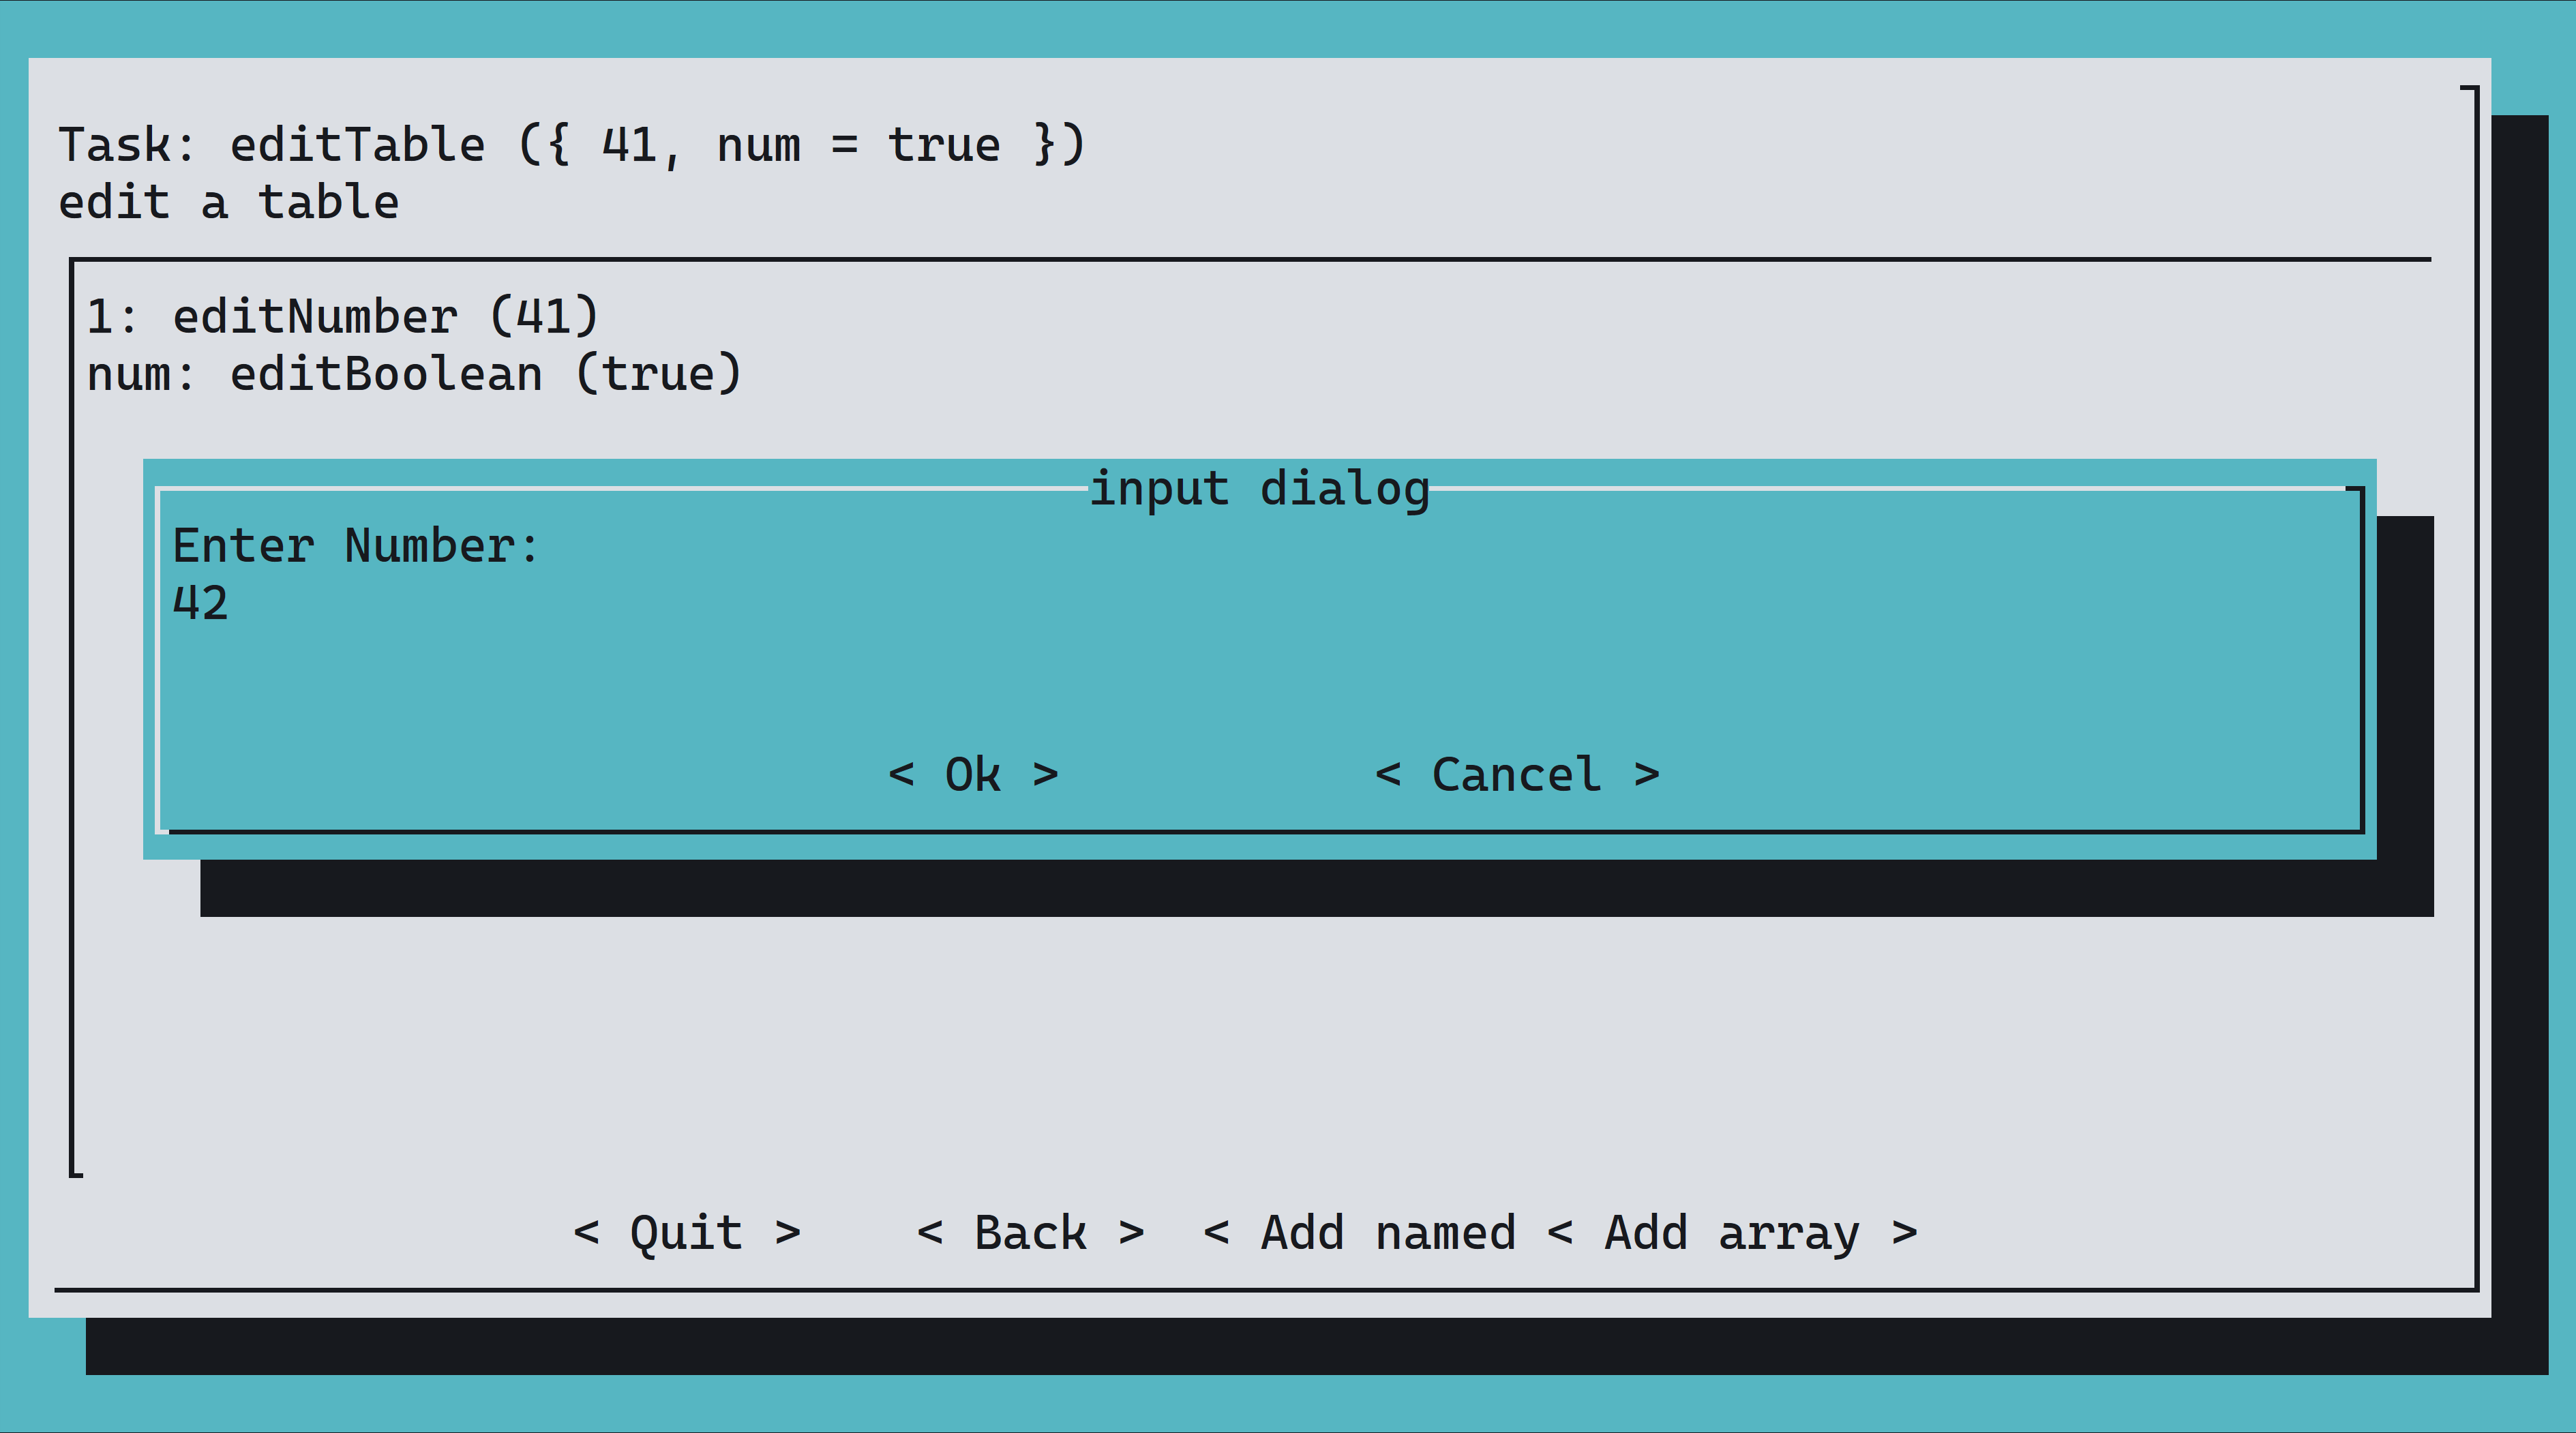
\includegraphics[width=0.8\textwidth]{img/screenshot-ltui.png}
%     \caption{The textual UI showing a table editor in the background with a number input dialog in the foreground.}
%     \label{fig:ltasks_ui}
% \end{figure}

% \newpage
\section{Wrap-up}\label{section-wrapup}
We explored a number of design decisions in this chapter, and decided on them for the LTasks implementation.
We defined that the proof-of-concept needs to have a basic implementation of tasks that can be composed sequentially and in parallel, and it needs to have editors with a UI (start of the chapter).
For handling typed tasks and editors, we decided to implement structural type matching (section \ref{section-types}).
We make use of coroutines by modelling the task as a table containing a coroutine, the task value and its stability (section \ref{section-task-values}).
The types are represented at runtime using the Typed library (section \ref{section-type-representation}).
We formalised a type specificity algorithm in section \ref{section-combinators-type-matching}. We noted what happens when lists or tables have more elements than required, and when lists have types in a different order than required.
For editors, we use a textual UI instead of a HTML page, a native application or a command-line application (section \ref{section-editors-ui}).
In the previous section (\ref{section-ltasks}) we show how the LTasks implementation works.

% \begin{itemize}
%     \item task types: structural type matching
%     \item task values: coroutine in table
%     \item type representation: Typed library
%     \item combinators, type matching
%     \item editor UI: text-based UI
%     \item LTasks implementation
% \end{itemize}


\chapter{Comparison}\label{comparison}
This chapter will compare iTasks and LTasks using a case study of the breakfast example adapted from Naus \cite{naus2020assisting} in listing \ref{lst:clean_breakfast}. To make it into a functioning example with editors, we need to modify it a bit. \lua{makeTea}, \lua{makeCoffee} and \lua{makeSandwich} are here modelled as editors. In the real world, they will be tasks that have no value initially, and a constant value once the tea, coffee or sandwich has been made. This allows us to make use of the standard task combinators without helper functions, like the example in listing \ref{lst:clean_breakfast}. This complete but contrived example is however more interesting because it makes use of editors and the transform combinator. The entire example can be seen in appendix \ref{appendix-breakfast}.

% \section{Main task and combinators}
The high level overview looks like listing \ref{lst:comparison_breakfast}. As you can see, they are almost identical. Lua uses different operators, and instead of an \clean{OnValue} there is a table with a \lua{fn} field.

\begin{figure}[ht]
\begin{subfigure}{\textwidth}
\centering
\begin{minted}{clean}
((makeTea -||- makeCoffee) -&&- makeSandwich) >>* [OnValue maybeEatBreakfast]
\end{minted}
\caption{In iTasks}
\label{lst:comparison_breakfast_clean}
\end{subfigure}
\begin{subfigure}{\textwidth}
\centering
\bigskip % space between subfigures
\begin{minted}{lua}
((makeTea | makeCoffee) & makeSandwich) ~ {{fn = maybeEatBreakfast}}
\end{minted}
\caption{In LTasks}
\label{lst:comparison_breakfast_lua}
\end{subfigure}
\caption{The main part of the breakfast example.}
\label{lst:comparison_breakfast}
\end{figure}

\section{Editors}
There is a bit more difference in making editors than in the basic combinators. iTasks uses combinators to add hints to editors, while LTasks includes the hints in the function signature, for simplicity. The most important difference in this example comes from the fact that Clean is statically typed, so the transformation function cannot return different types as in Lua. Instead, it has to return a maybe (an algebraic data type), and we need to use \clean{tvFromMaybe}, which takes a \clean{TaskValue} of a \clean{?None} or \clean{?Just} and turns it into \clean{NoValue} or \clean{Value}, respectively. This is not needed in LTasks, where we can simply return \lua{nil} from the transformation function.

\begin{figure}[ht]
\begin{subfigure}{\textwidth}
\centering
\begin{minted}{clean}
makeTea = updateInformation [] False <<@ Hint "Make tea?"
        @ (\x -> if x (?Just "Tea") ?None)
        @? tvFromMaybe
\end{minted}
\caption{In iTasks}
\label{lst:comparison_editors_clean}
\end{subfigure}
\begin{subfigure}{\textwidth}
\centering
\bigskip % space between subfigures
\begin{minted}{lua}
local makeTea = editor.editBoolean(false, "make tea?")
    :transformValue(function(x) return x and "Tea" or nil end)
\end{minted}
\caption{In LTasks}
\label{lst:comparison_editors_lua}
\end{subfigure}
\caption{Making a boolean editor that results in either ``Tea'' or nothing.}
\label{lst:comparison_editors}
\end{figure}

\section{Helper function}
Listing \ref{lst:comparison_maybe} shows the helper functions that are needed in order to create a \lua{viewInformation} task only if both a food and a drink are chosen.
These functions are written differently because in iTasks we use the maybe type and pattern matching, while we use \lua{nil} in LTasks.

\begin{figure}[ht]
\begin{subfigure}{\textwidth}
\centering
% maybeEatBreakfast :: (TaskValue (String, String)) -> ? (Task String)
\begin{minted}{clean}
maybeEatBreakfast (Value (drink, food) _) = ?Just (eatBreakfast drink food)
maybeEatBreakfast _ = ?None
\end{minted}
\caption{In iTasks}
\label{lst:comparison_maybe_clean}
\end{subfigure}
\begin{subfigure}{\textwidth}
\centering
\bigskip % space between subfigures
\begin{minted}{lua}
local function maybeEatBreakfast(value)
    if value[1] ~= nil and value[2] ~= nil then
        return eatBreakfast(value[1], value[2])
    end
end
\end{minted}
\caption{In LTasks}
\label{lst:comparison_maybe_lua}
\end{subfigure}
\caption{Making a boolean editor that results in either "Tea" or nothing.}
\label{lst:comparison_maybe}
\end{figure}

\section{User interface}
The user interface for LTasks (shown in figure \ref{fig:comparison_ltask_ui}) is made to serve two purposes: to be the bare minimum for a TOP proof-of-concept, and to make clear that the behaviour is correct for TOP. For that reason, it looks very different to the iTasks UI.

Let us set aside the differences in visual display for now (LTasks uses a textual UI while iTasks uses a webpage). The textual UI of LTasks shows the structure of the task at the top. This is not only useful for seeing that the structure is indeed correct, but also for keeping a mental image of where you are navigated to. This is not necessary in iTasks because it shows everything at once instead of entering sub-menus (fig. \ref{fig:comparison_itask_ui}). iTasks hides the way in which \lua{makeTea} and \lua{makeCoffee} are composed with \lua{makeSandwich}, while the LTasks UI makes this more explicit.

\begin{figure}
\centering
\begin{subfigure}{0.45\textwidth}
    \centering
    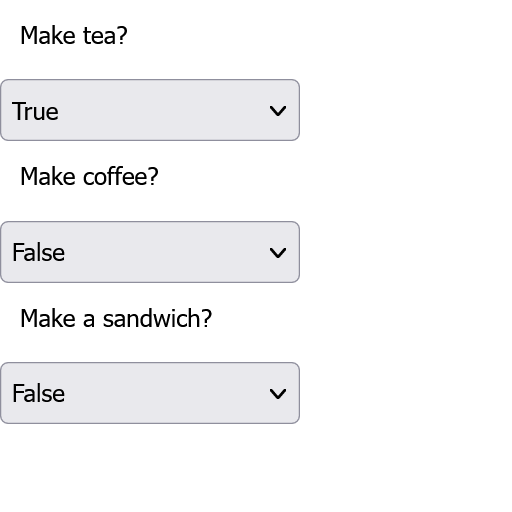
\includegraphics[width=\textwidth]{img/screenshot-itasks-breakfast.png}
    \caption{The UI showing all input fields at once.}
    \label{fig:comparison_itask_ui_1}
\end{subfigure}
\hspace{0.05\textwidth}
\begin{subfigure}{0.45\textwidth}
    \centering
    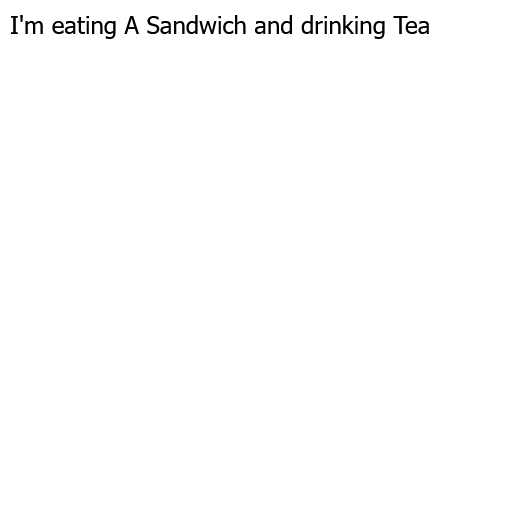
\includegraphics[width=\textwidth]{img/screenshot-itasks-breakfast-view.png}
    \caption{The UI showing the output after selecting \lua{true} for \lua{makeSandwich}.}
    \label{fig:comparison_itask_ui_2}
\end{subfigure}
\caption{The graphical web UI of iTasks.}
\label{fig:comparison_itask_ui}
\end{figure}

\begin{figure}
\centering
\begin{subfigure}{0.8\textwidth}
    \centering
    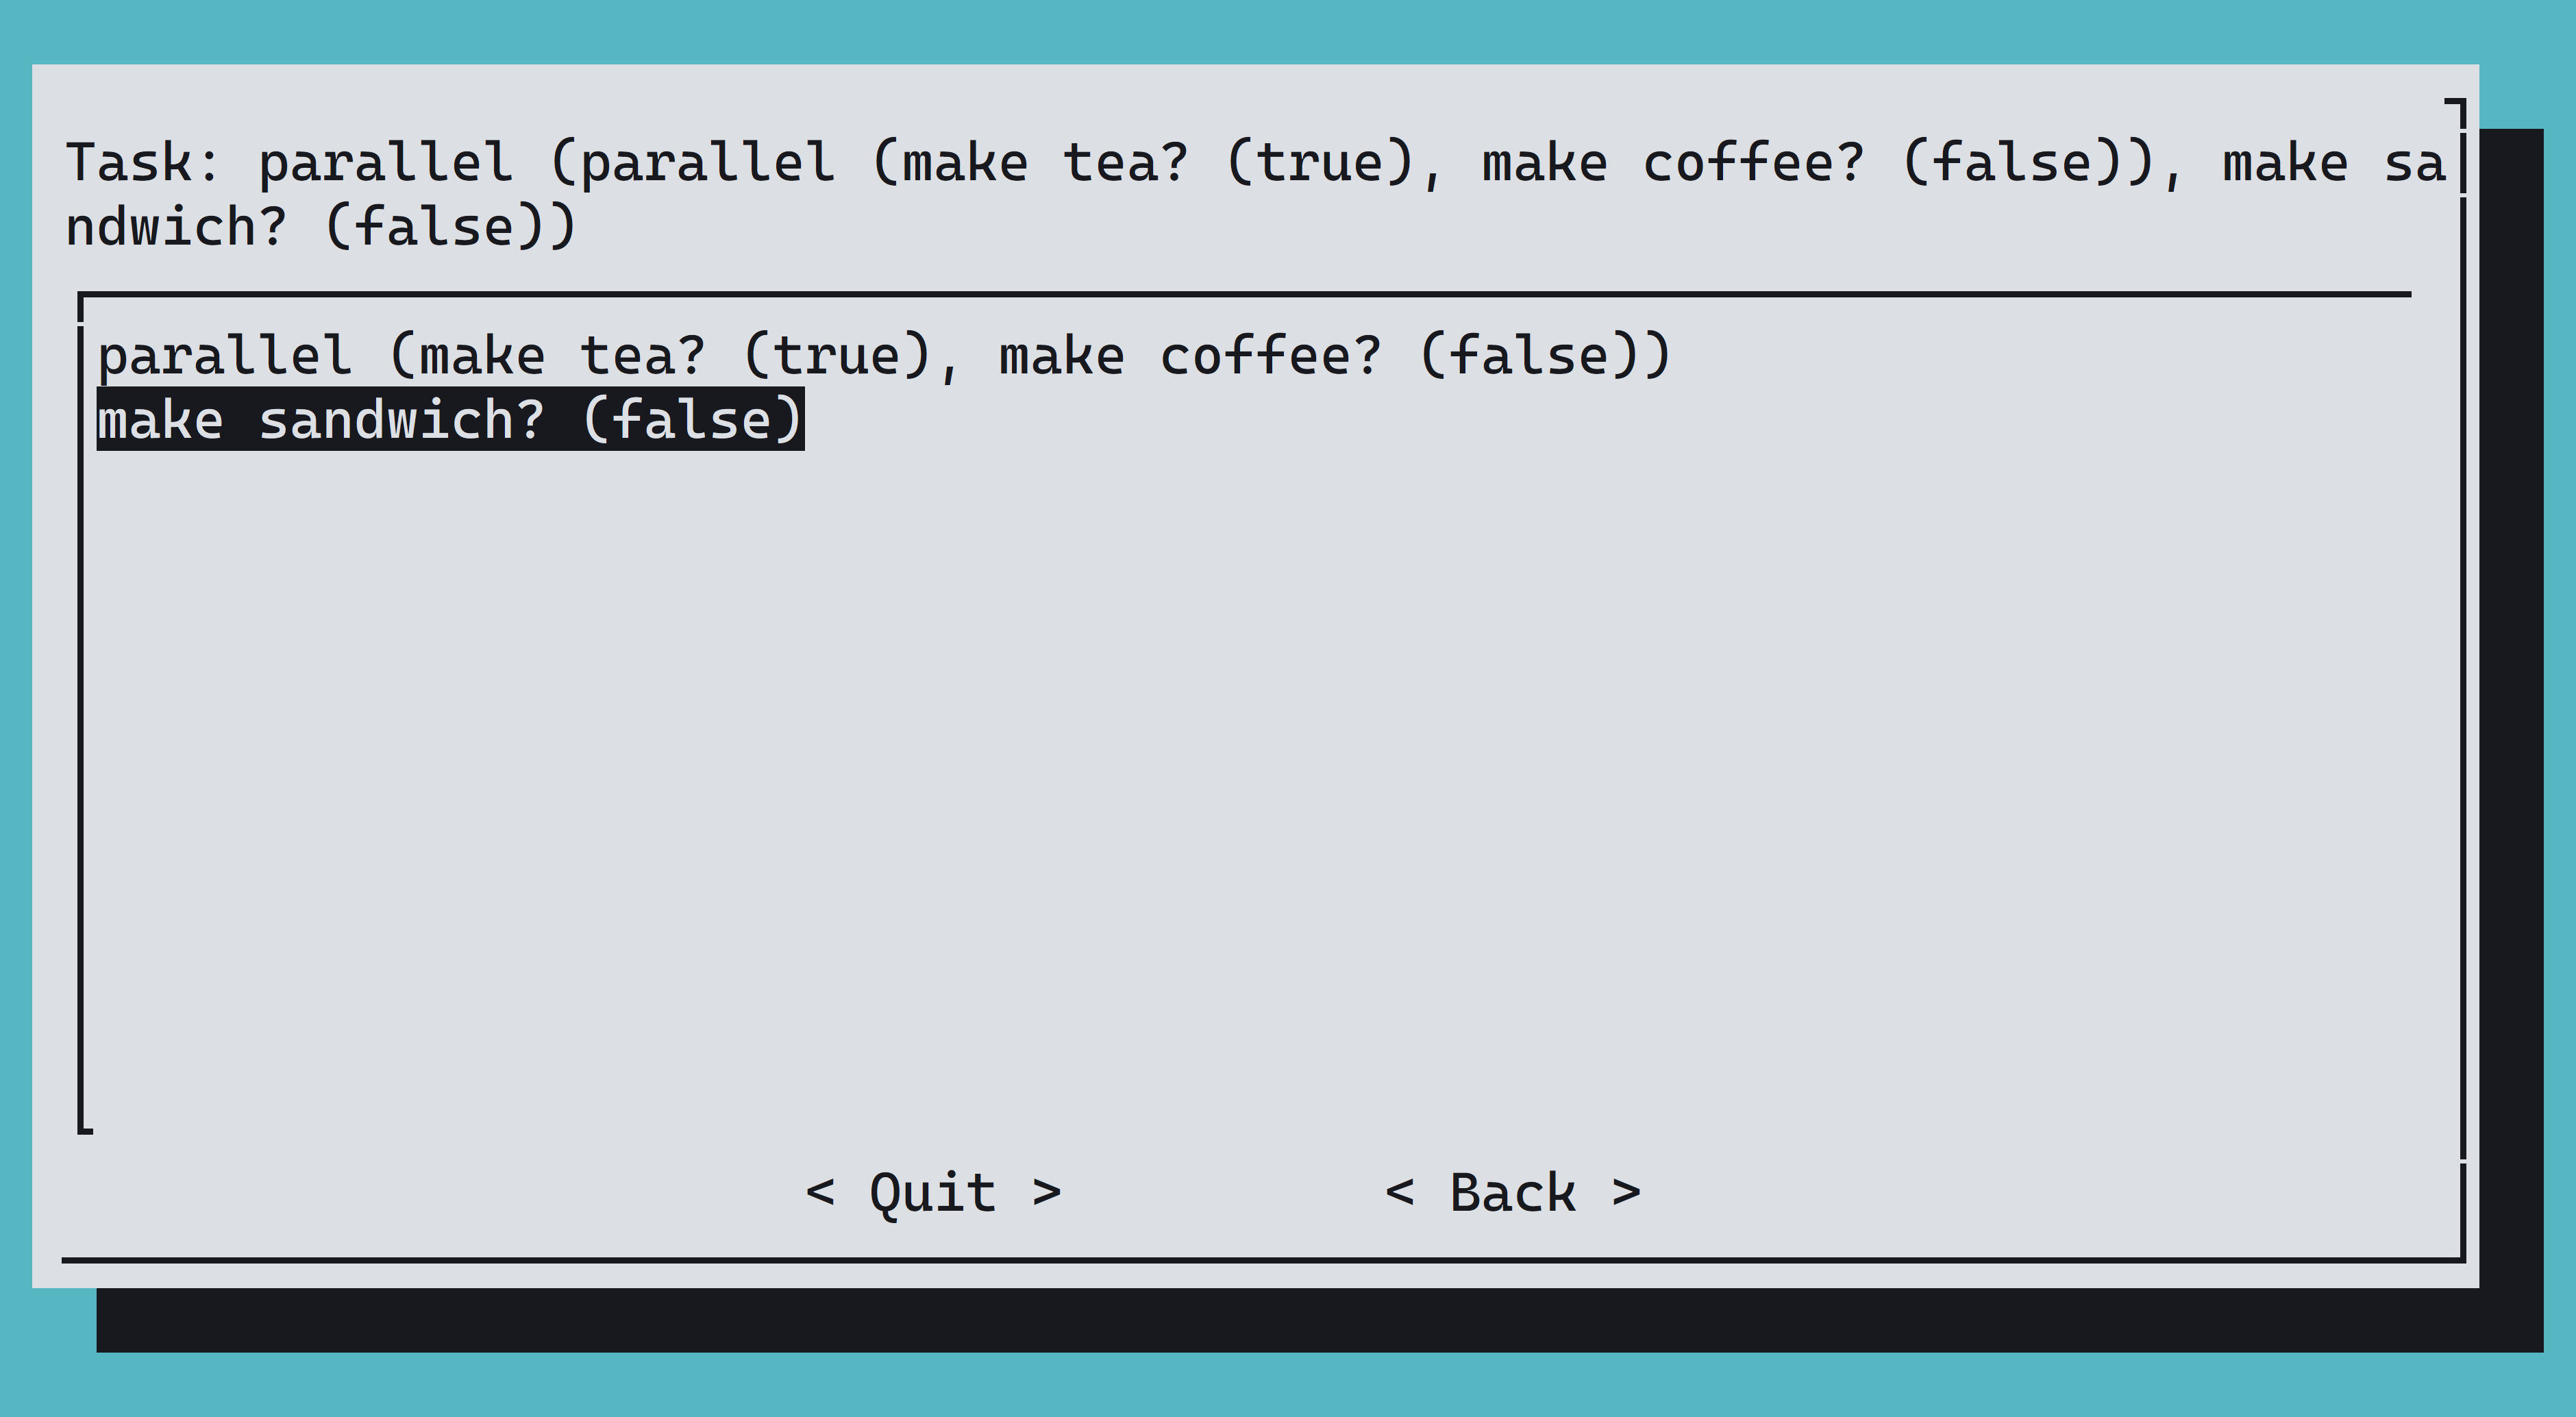
\includegraphics[width=\textwidth]{img/screenshot-ltasks-breakfast.png}
    \caption{The UI showing that \lua{makeTea} is \lua{true} and that \lua{makeCoffee} and \lua{makeSandwich} (selected) are both \lua{false}.}
    \label{fig:comparison_ltask_ui_1}
\end{subfigure}
\begin{subfigure}{0.8\textwidth}
    \centering
    \bigskip
    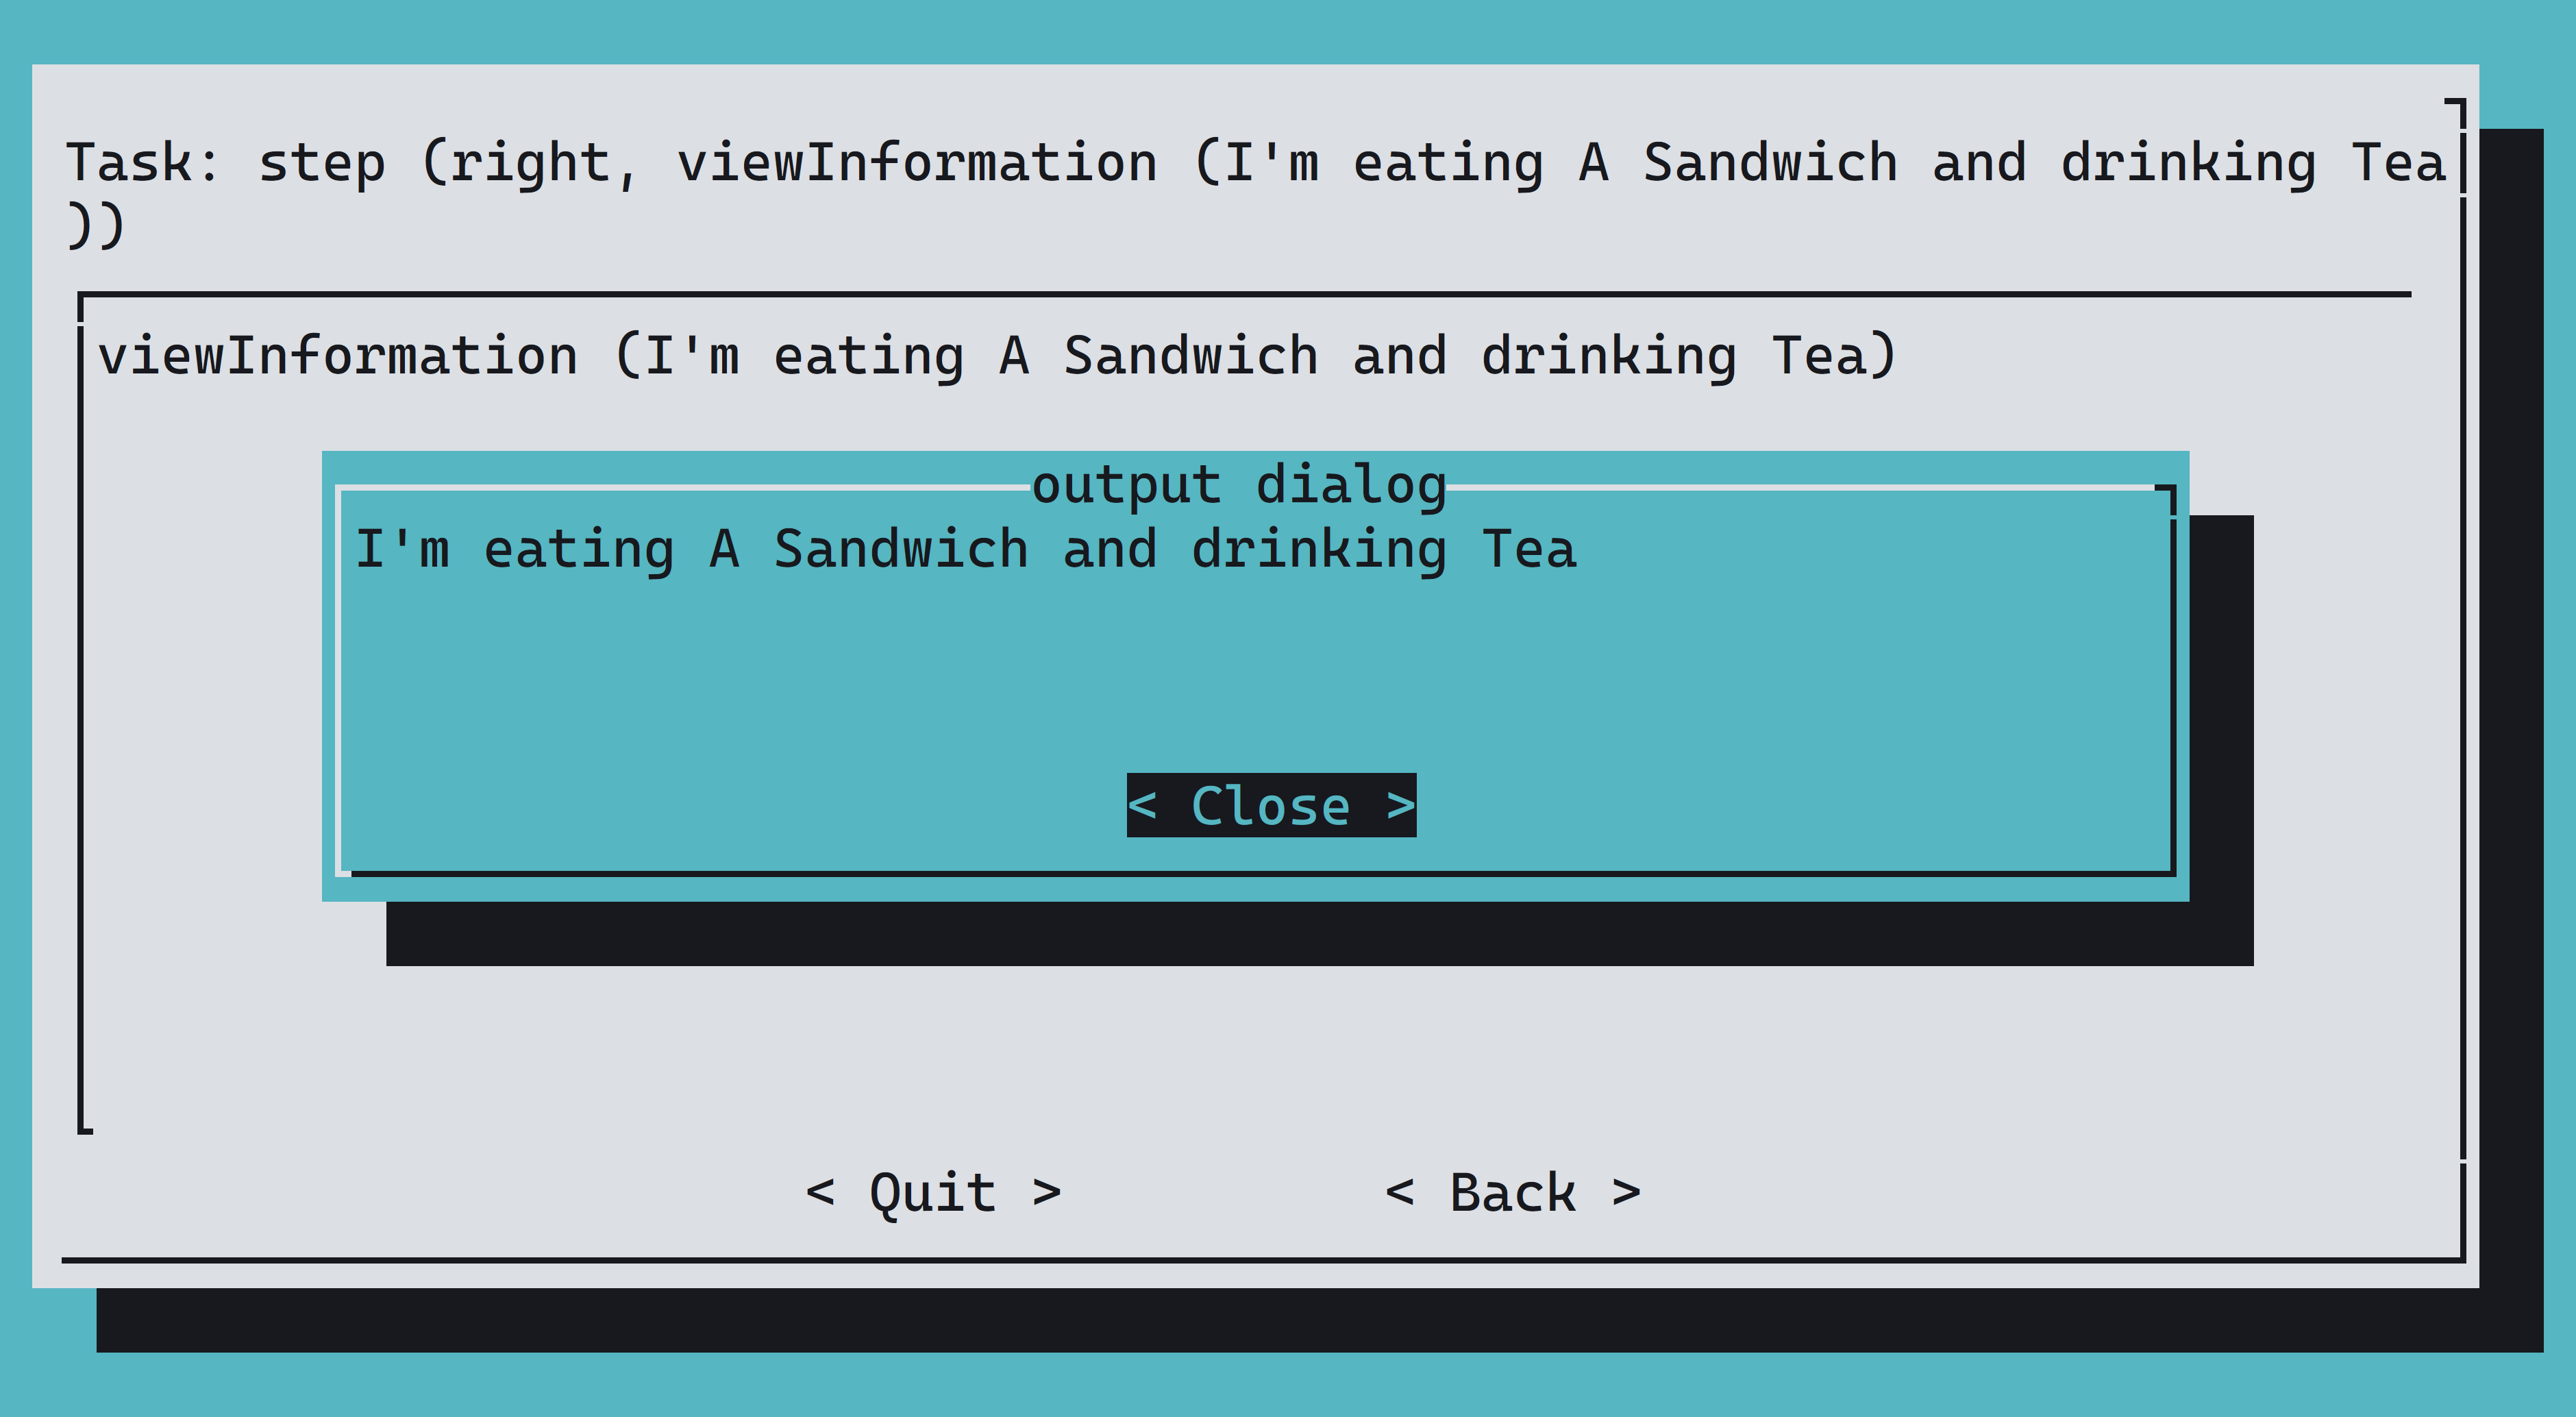
\includegraphics[width=\textwidth]{img/screenshot-ltasks-breakfast-view.png}
    \caption{The UI showing the output after selecting \lua{true} for \lua{makeSandwich}.}
    \label{fig:comparison_ltask_ui_2}
\end{subfigure}
\caption{The textual UI of LTasks.}
\label{fig:comparison_ltask_ui}
\end{figure}

\section{When to use which}
In general, LTasks is more suited for problems that have a large dynamic aspect, and for quick prototyping. Such a dynamic problem can be allowing users to enter a date in multiple formats. It is useful for quick prototyping, because you do not need to first define the types and derive the right classes, as you would in iTasks (see the date example in \ref{appendix-dates-itasks}).

Bringing TOP to Lua is not all sunshine and roses, though. The small standard library of Lua means that you need to define some functions yourself, while they are provided in Clean. In the date example (\ref{appendix-dates}), Clean has the \clean{elemIndex} function, which needs to be defined manually with LTasks. We disregard the \clean{parseDate} function added by iTasks here, because LTasks is only a proof of concept. Lastly, while Lua is more free in what you can do, Clean---being statically typed---provides some static guarantees, which is important in some situations.

\chapter{Related Work}\label{relatedwork}
In this chapter you demonstrate that you are sufficiently aware of the
state-of-art knowledge of the problem domain that you have investigated as
well as demonstrating that you have found a \emph{new} solution / approach / method.

iTasks: \cite{plasmeijer2007itasks}

mTasks: \cite{koopman2018task, lubbers2019multitasking}

\chapter{Conclusions}\label{conclusions}
% In this chapter you present all conclusions that can be drawn from the
% preceding chapters.
% It should not introduce new experiments, theories, investigations, etc.:
% these should have been written down earlier in the thesis.
% Therefore, conclusions can be brief and to the point.

In this bachelor thesis we explored the design decisions that come up when implementing TOP in the procedural language Lua, and we have written a proof-of-concept TOP implementation called LTasks.
LTasks contains the most important parts for a TOP implementation: it has tasks, these tasks can be composed sequentially and in parallel, and there is interaction with users through editor tasks.

The first major difference between Clean and Lua is that Clean is statically typed while Lua is dynamically typed.
We explored a number of ways to work with Lua's dynamic types. Structural type matching is the most interesting choice here, which we use in LTasks.
% : adding types, using validator and conversion functions, interfacing with JSON APIs or structural type matching.
% The second major difference between Clean and Lua is that
Lua has coroutines while Clean does not. Coroutines are more convenient than functions for modelling tasks, so a task in LTasks is a table with a coroutine.
The most important choice for structural type matching is whether to choose the first match or the best match. We defined an algorithm to find that best match, which we use in LTasks.
User interaction through editors in LTasks happens in a text-based user interface, because that is the simplest form of UI that can display all TOP features.

% There are a number of ways to do structural type matching for the step continuation tasks. We can either choose first match or the best match, and we defined an algorithm to find that best match. We defined that lists that are longer or that have a different order of types should not match, and that tables with more fields should match.

% For editors, we can create a HTML page, a native application, a text-based UI or a command-line UI.

% For LTasks, we chose to do structural type matching. Tasks are modelled as tables containing coroutines. We use the Typed library to represent and match types, but use our own algorithm for finding the most specific type. We use the LTUI library for creating a text-based UI.

\section{Future work}
The proof-of-concept implementation uses the Typed library to represent types at runtime. However, this library can only represent a limited set of data structures and is very strict in what it matches. Further research could find a better way of representing types at runtime so that more Lua features can be used, developing a less strict type matching algorithm and a more complete type specificity relation to go along with it. One can look at Typed Lua \cite{maidl2014typed} or Pallene \cite{gualandi2020pallene} as inspiration for the types.

This research focused only on the core concepts of TOP, and left shared data sources and exceptions out of scope. Further research can go to expanding the LTask implementation by bringing SDS and exceptions to Lua.

% A better way of representing types so that more Lua features can be used. Since the main goal of using types here is not to check the correctness of a program but to use them for augumenting the features Lua provides, the ``type system'' should not aim for soundness but rather for completeness.
% Related to this, a custom type matching algorithm and a more complete type specificity algorithm.


\bibliographystyle{plain}
\bibliography{bibliography}

% reset verbatim environment for appendix, otherwise minted pagebreaks and linenos are broken
\RecustomVerbatimEnvironment{Verbatim}{Verbatim}{}

\appendix
\chapter{Examples in LTasks and iTasks}\label{appendix-examples}
% Appendices are \emph{optional} chapters in which you cover additional material that is required to support your
% hypothesis, experiments, measurements, conclusions, etc. that would otherwise
% clutter the presentation of your research.

This appendix contains full code of examples using both iTasks and LTasks, in order for comparing them. \ref{appendix-breakfast} shows the full code for the breakfast example used throughout this thesis. \ref{appendix-dates} shows an additional example of letting the user input multiple date formats.

\section{Breakfast}\label{appendix-breakfast}
\subsection{In LTasks}
\inputminted{lua}{examples/breakfast.lua}

\subsection{In iTasks}
\inputminted{clean}{examples/breakfast.icl}

\newpage
\section{Multiple date input formats}\label{appendix-dates}
\subsection{In LTasks}
\inputminted{lua}{examples/date.lua}

\subsection{In iTasks}
\inputminted{clean}{examples/date.icl}

\chapter{LTask code}\label{appendix-ltask}
The full code repository can be found at \url{https://github.com/Dantevg/LTasks}, the three most important files for this thesis are attached here: \lua{task.lua} in \ref{appendix-ltask-task.lua}, \lua{types.lua} in \ref{appendix-ltask-types.lua} and \lua{ltuiEditor.lua} in \ref{appendix-ltask-ltuiEditor.lua}.

\section{task.lua}\label{appendix-ltask-task.lua}
\inputminted[linenos]{lua}{code/task.lua}

\section{types.lua}\label{appendix-ltask-types.lua}
\inputminted[linenos]{lua}{code/types.lua}

\section{ltuiEditor.lua}\label{appendix-ltask-ltuiEditor.lua}
\inputminted[linenos]{lua}{code/ltuiEditor.lua}


\end{document}
